%%%%%%%%%%%%%%%%%%%%%%%%%%%%%%%%%%%%%%%%%%%%%%%%%%%%%%%%%%%%
% Manuscript started: 2007/09/01
% First draft: 2008/02/??, Vitamin D, Inc.
%%%%%%%%%%%%%%%%%%%%%%%%%%%%%%%%%%%%%%%%%%%%%%%%%%%%%%%%%%%%

\documentclass[oneeqnum,onefignum,onetabnum,onethmnum]{siamltex}
\usepackage{graphics}
\usepackage{multirow}

% Macros for entire document

% Utility commands
\newcommand{\bc}{\begin{center}}
\newcommand{\ec}{\end{center}}
\newcommand{\beq}{\begin{equation}}
\newcommand{\eeq}{\end{equation}}
\newcommand{\bea}{\begin{eqnarray}}
\newcommand{\eea}{\end{eqnarray}}
\newcommand{\ba}{\begin{array}}
\newcommand{\ea}{\end{array}}

% Fancy equation environments
\newcommand{\Eq}[2][Eq.~]{{#1}(\ref{eq:#2})}                                    
\newcommand{\Eqs}[1]{Eqs.~(\ref{eq:#1})}                                        
\newcommand{\Fig}[2][Fig.~]{{#1}\ref{fig:#2}}                                   
\newcommand{\Figs}[1]{Figs.~\ref{fig:#1}}                                       
\newcommand{\Sec}[2][Sec.~]{{#1}\ref{sec:#2}}                                   
\newcommand{\Secs}[1]{Secs.~\ref{sec:#1}}      

% Common expressions
\def\eg{\emph{e.g., }}
\def\ie{\emph{i.e., }}
\def\etal{\emph{et al.}}
\def\etc{\emph{etc.}}

% Mathematical notation
\def\div{\ensuremath{\nabla \cdot}}
\def\divs{\ensuremath{\nabla_{s} \cdot}}
\def\grad{\ensuremath{\nabla}}
\def\grads{\ensuremath{\nabla_{s}}}
\def\lapl{\ensuremath{\nabla^2}}
\def\Real{\ensuremath{\mathrm{Re}}}
\newcommand{\tensor}[1]{\ensuremath{{\bf{#1}}}}

\newcommand{\ddx}[2]{\frac{\partial #1}{\partial #2}}
\newcommand{\DDx}[2]{\frac{D #1}{D #2}}
\newcommand{\sgn}[1]{\ensuremath{\mathrm{sgn}(#1)}}
\newcommand{\abs}[1]{\ensuremath{\left|#1\right|}}


% MATH MACROS
\def\sech{\mathrm{sech}}
\def\erfc{\mathrm{erfc}}

% PDE MACROS
\def\pt{\partial t}
\def\px{\partial x}
\def\py{\partial y}
\def\tu{\tilde{u}}

% NUMERICS MACROS
\def\dt{\Delta t}
\def\dx{\Delta x}
\def\dy{\Delta y}
\def\dy{\Delta y}
\def\dto{\dt_{opt}}


\title{Using Optimal Time Step Selection to Boost the Accuracy of
       Finite Difference Methods for a Class of 
       Time Dependent Partial Differential Equations}

\author{
Kevin T. Chu\footnotemark[2]
}

\begin{document}
\bibliographystyle{unsrt}
\maketitle

\renewcommand{\thefootnote}{\fnsymbol{footnote}}
\footnotetext[2]{Vitamin D, Inc., Menlo Park, CA 94025} 

\renewcommand{\thefootnote}{\arabic{footnote}}


\begin{abstract}
In this article, we discuss a novel technique based on optimal time step 
selection for boosting low-order finite difference schemes
into higher-order numerical methods for time dependent partial differential
equations (PDEs).  We demonstrate the utility of this technique on several 
classical hyperbolic and parabolic problems in one and more space dimensions 
and explain the observed orders of convergence through straightforward numerical
analysis arguments.
** HIGH-ORDER PDES AND IRREGULAR DOMAINS ***
\end{abstract}


\begin{keywords}
optimal time step, finite difference methods, high-order accuracy, 
time dependent PDEs, initial-value problems
\end{keywords}

\begin{AMS}
65-02, 65M06, 65M12, 65M20
\end{AMS}

\pagestyle{myheadings}
\thispagestyle{plain}
\markboth{KEVIN T. CHU}
         {HIGH-ORDER ACCURATE FD SCHEMES VIA OPTIMAL TIME STEP SELECTION} 


\section*{Introduction}
High-order numerical methods for partial differential equations (PDEs) will 
always be valuable for increasing the computational efficiency of numerical 
simulations.  Thus, it is not at all surprising that a great deal of effort in 
numerical PDEs continues to be focused on the development of high-order 
numerical schemes~\cite{gibour_2005,??}.  
Typically, high-order accuracy is achieved by constructing
schemes that have high formal orders of accuracy.  However, high-order 
accurate numerical solutions can also be obtained by using formally low-order 
schemes in clever ways.  When possible, the latter approach can be a powerful 
way to boost the accuracy of a numerical method \emph{without} introducing too 
much additional algorithmic (and programming) complexity.

High-order accurate methods that are simple combinations or modifications of 
low-order schemes abound.  A few well-known examples include Richardson 
extrapolation~\cite{richardson_1927,heath_book}, the modified nine-point 
formula for the Poisson equation~\cite{iserles_book}, and the Lax-Wendroff 
method for the advection equation~\cite{leveque_book_1992, leveque_book_2002,
gko_book}.  Cancellation of higher-order errors (whether fortuitous or 
intentional) is a key to principle underlying the superior accuracy of these 
each of methods.

More commonly, high-order accurate numerical methods are constructed by 
requiring that the discretization error possesses the desired formal order of 
accuracy for \emph{all} of the independent variables in the PDE.  While this 
constraint is certainly sufficient for high-order accuracy, it is by no means 
necessary.  This standard approach for developing numerical methods for PDEs 
has its roots in the classical numerical analysis of PDEs, which tends to 
individually analyze the discretization of the terms in the PDE.  Within this 
framework, it is natural to seek high-order accuracy by ensuring that the 
numerical scheme is simultaneously high-order accurate for \emph{all} 
independent variables.  Unfortunately, this common approach for developing 
and analyzing numerical methods is often suboptimal because it neglects the 
potential for achieving high order of accuracy using only simple finite 
difference schemes based on compact, low-order stencils.

Perhaps the greatest weakness of the standard method for constructing 
high-order numerical methods is the use of ``big-O" notation, which hides all 
of the details about higher-order errors.  The information lost in the ``big-O" 
notation eliminates the possibility of reducing numerical error by taking 
advantage of relationships between the terms in the error.  The modified 
nine-point formula for the Poisson equation (also known under the name 
Mehrstellen)~\cite{iserles_book} and the Lax-Wendroff scheme for the 
advection equation~\cite{leveque_book_1992, leveque_book_2002, gko_book} 
demonstrate the power of explicitly retaining higher-order terms in the 
discretization error when analyzing numerical schemes.  For both of these 
methods, examination of higher-order terms allows low-order methods to be 
transformed into high-order methods with only minor modifications to the 
numerical scheme.  

The usual approach for developing numerical methods has another significant
shortcoming -- it places no value on optimization of numerical parameters 
(\eg $\dx$ and $\dt$) for accuracy.  Again, ``big-O" notation is 
somewhat to blame for this situation because it gives the false impression 
that the error depends on each numerical parameter independently.  Aside
from constraints needed for numerical stability, ``big-O" notation makes 
it appear as though any combination of numerical parameters is equally good 
as long as they are all ``small enough.''  For some problems, however, 
optimizing the numerical parameters can significantly increase the accuracy
of the numerical solution.  For example, in~\cite{zhao_2006} Zhao showed 
that appropriately choosing the value of $\theta$ as a function of the time 
step, $\dt$, in the theta-method\footnote{In~\cite{zhao_2006} refers 
to $\theta$ as the weight factor and the theta-method as the single-step 
trapezoidal method.}~\cite{iserles_book, gko_book} can decrease the error 
of finite element solutions to the diffusion equation. 

In this paper, we explore a novel technique based on optimal time step (OTS)
selection that can be used to construct high-order finite difference schemes 
for time dependent PDEs using only formally low-order stencils.  The essential 
idea is that a carefully chosen time step (and possibly the addition of
a few correction terms) can eliminate low-order terms in the discretization 
error, allowing a formally low-order method to deliver high-order accuracy.  
The optimal time step is calculated through a straightforward analysis of the 
discretization error that uses information from the PDE to relate the 
leading-order terms.  Optimal time step selection combines the well-known 
approach of using information provided by the PDE to reduce numerical error 
with the less-common notion that optimal choice of numerical parameters can 
boost the effectiveness of algorithmically simple and computationally 
low-cost methods.  

Using the PDE being solved to reduce discretization error has a long 
tradition in numerical analysis.  Indeed, this idea underlies both the 
modified nine-point formula for the Poisson equation~\cite{iserles_book} and 
the Lax-Wendroff method for the linear advection 
equation~\cite{leveque_book_1992, leveque_book_2002, gko_book}.  
In the case of the modified nine-point formula for the Poisson equation, a 
simple analysis of the nine-point stencil for the Laplacian on a uniform grid 
shows that it is only second-order, which might lead to the conclusion that 
the nine-point stencil has no advantage over the standard five-point stencil.  
However, a more careful analysis of the discretization error in light of the 
PDE reveals that the leading-order error, which is proportional to the 
bilaplacian of the solution~\cite{iserles_book, patra_2005}, is directly 
related to the Laplacian of the source term in the Poisson equation.  Thus, 
the numerical scheme is easily boosted to fourth-order by simply adding a 
correction term that cancels out the leading-order error.   
Similarly, use of the PDE to eliminate higher-order discretization errors also 
plays a critical role in the Lax-Wendroff method because it allows the second 
derivative of the solution in time to be written in terms of the second 
derivative in space.  This observation transforms an unstable, first-order 
scheme based on a central difference approximation of 
$\partial/\partial x$ into a stable, second-order 
scheme~\cite{leveque_book_1992, leveque_book_2002}.

Optimal time step selection as a technique for improving the overall accuracy 
of numerical schemes for time dependent PDEs appears to be a novel idea.
Typically, the primary concern when choosing a time step is numerical 
stability with accuracy being a secondary consideration.  The fact that a 
clever choice of time step can be used to dramatically reduce the error is 
rarely considered.  In general, little research seems to have been done on 
optimizing the parameters of numerical methods (\eg time step and grid 
spacing) to improve accuracy.  To the best of the authors knowledge, Zhao's 
method for choosing an optimal value of $\theta$ in the theta-method is the 
only work that attempts to improve accuracy by modifying numerical parameters.
While he focuses solely on the optimal choice of $\theta$ for a fixed time 
step, his approach can be viewed as a form of optimal time step selection by 
reversing the roles of $\theta$ and the time step.  

Before moving on, it is worth spending a few moments to draw the distinction
between optimal time step selection and traditional adaptive time stepping 
techniques~\cite{iserles_book,??} that are used in the context of the method 
of lines~\cite{iserles_book, gko_book}.  On the surface, optimal time step 
selection may appear to be just a crude version of adaptive time step control.
However, the two methods are actually very different.  While both methods seek 
to reduce numerical error by controlling the time step, the numerical errors 
they control are fundamentally different.  Adaptive time stepping can only 
be used to reduce temporal discretization errors because it controls the 
errors that arise when solving the coupled system of ODEs for the 
semi-discrete approximation to the PDE; the spatial discretization errors 
are completely controlled by the finite difference scheme selected to 
approximate the spatial derivatives.  
In contrast, optimal time step selection simultaneously reduces 
\emph{both} the spatial and temporal discretization errors because it
uses information from the PDE to choose the time step.  Thus, optimal time 
step selection has the potential to produce superior results compared with 
traditional adaptive time stepping approaches for integrating the 
semi-discrete equations associated with time dependent PDEs.  Another 
important distinction between the two techniques is that optimal time step 
selection uses a \emph{fixed} time step which makes it significantly less 
computationally complex than adaptive time stepping methods.

As a technique for constructing numerical methods, optimal time step selection 
has several desireable features.  Like any technique that leads to high-order 
methods, optimal time step selection produces schemes that greatly reduce the 
computational cost required to obtain a numerical solution of a desired 
accuracy.  However, its real power comes from the fact that it achieves
high-order accuracy while being based solely on very simple finite difference 
schemes.  For instance, we will see how optimal time step selection makes 
it possible to achieve 4th-order accuracy for the diffusion equation using only 
a second-order stencil for the Laplacian and forward Euler time integration.  
Moreover, high-order accuracy is not restricted to problems on simple, 
rectangular domains; irregular domains are straightforward to handle by
appropriately setting the values in ghost cells~\cite{fedkiw_1999, 
osher_fedkiw_book, gibou_2005}.  Optimal time step selection is even 
beneficial when using finite difference schemes to solve some nonlinear PDEs.  
While there are certainly limitations to optimal time step selection, we will 
see that there are a many problems where it is useful.  

The remainder of this paper is organized as follows.  
In Section~\ref{sec:optimal_time_step_selection}, we begin by 
discussing the technique of optimal time step selection in detail and 
presenting the analysis that shows how it boosts the order of accuracy 
for formally low-order numerical schemes.  In 
Section~\ref{sec:applications_1d}, we demonstrate the general utility of 
optimal time selection to problems in one space dimension by applying it to 
finite difference schemes for several classical linear and nonlinear PDEs. 
In Section~\ref{sec:applications_multidim}, we use optimal time step selection 
to improve the accuracy of simple finite difference schemes for the linear 
advection equation and diffusion equation in multiple space dimensions.  
To illustrate the ease with which high-order accuracy can be achieved for
problems on arbitrary domains, the 2D diffusion equation is solved on both 
the regular and irregular domains.  
For each PDE in Sections~\ref{sec:applications_1d} and 
\ref{sec:applications_multidim}, we provide the numerical analysis required 
to calculate the optimal time step size and order of accuracy.  
Finally, in Section~\ref{sec:summary}, we provide some concluding remarks on 
the applicability and limitations of optimal time step selection for the 
numerical solution of general time dependent PDEs.  


\section{\label{sec:optimal_time_step_selection} 
         Optimal Time Step Selection}
Optimal time step selection is not by itself a method for constructing 
finite difference schemes.  Rather it is a way to enhance to the performance
of existing finite difference schemes by carefully choosing the time step to 
eliminate low-order numerical errors.  The two basic ideas underlying 
optimal time step selection are (1) the PDE provides valuable insight into the 
discretization errors for finite difference schemes and (2) a judicious choice 
of time step can be used to eliminate the leading-order (and possibly 
higher-order) terms in the error.  In this section we present and analyze the 
technique of optimal time step selection for finite difference schemes 
constructed to solve evolution equations of the form 
$\frac{\partial u}{\partial t} = \ldots$, where the right hand side only 
involves functions of the independent variable and its spatial derivatives.  
Because this class of time dependent PDEs is so prevalent and important in 
many problems of applied mathematics, restricting our attention to problems 
of this form is not a serious limitation.  


\subsection{\label{sec:ots_model_pde} 
            Optimal Time Step for a Model PDE}
Let us begin by considering a finite difference approximation to a 
time dependent PDE of the form
\beq
  \frac{\partial u}{\partial t} = A \frac{\partial^n u}{\partial x^n},
  \label{eq:model_PDE}
\eeq
where $u$ is the solution to the PDE, $n$ is the spatial order of the 
PDE, and $A$ is a constant of the appropriate sign so that~(\ref{eq:model_PDE}) 
is well-posed.  Because we will be boosting the accuracy of the FD 
approximation by optimizing the time step, there is no reason to explicitly
construct the scheme to be high-order.  In fact, using a high-order FD scheme 
only complicates the analysis required to calculate the optimal time 
step.  

To compute the optimal time step, we first analyze the discretization errors 
(both spatial and temporal) for the FD approximation, explicitly keeping track 
of the leading-order terms.  In contrast to standard error analysis, we do 
not sweep all of the errors under ``big-O'' notation.  Rather, we take 
advantage of the fact that derivation of the leading-order terms in the 
error is straightforward for FD schemes through the use of Taylor series 
expansions.  Because each term in the error is proportional to a partial 
derivative of the solution, we can attempt to use the PDE to relate the 
leading-order terms to each other.  If we are fortunate (which in many cases 
we are), this careful analysis yields a direct relationship between the 
leading-order spatial and temporal errors that allows them to be combined as 
a single term of the form:
\beq
  (L u) P(\dx, \dt) ,
  \label{eq:leading_order_error_model_PDE_general}
\eeq
where $P$ is a polynomial in the numerical parameters, $L$ is a differential 
operator, $u$ is the solution to the PDE, and we have assumed that the 
grid spacing is equal in all spatial directions\footnote{In general, the grid 
spacing need not be equal in all spatial directions.  For some problems, it is 
only possible to calculate an optimal time step if the grid spacing is
unequal between the different spatial directions.}.  By selecting the 
numerical parameters so that $P = 0$, we can completely eliminate the 
leading-order term in the discretization error.  Because time dependent PDEs 
are often solved by stepping in time, it is natural to choose the time step 
to be a function of the grid spacing.  The time step selected in this way 
is the \emph{optimal time step} for the finite difference scheme.  

An important class of FD schemes for time dependent PDEs are those based
on the method of lines.   When the method of lines approach is used for 
(\ref{eq:model_PDE}), $P$ takes a particularly simple 
form:
\beq
  P(\dx, \dt) = (\alpha \dx^r - \beta \dt^s) \dt,
  \label{eq:leading_order_error_model_PDE_MOL}
\eeq
where $r$ and $(s+1)$ are the orders of the leading spatial and temporal 
errors, and $\alpha$ and $\beta$ are positive constants that depend on the 
details of the PDE and FD scheme.  Setting $P = 0$, we find that the optimal 
time step is given by\footnote{The $\dt = 0$ root of $P$ is discarded 
because it is not numerically meaningful.}
\beq
  \dto = \gamma \dx^{r/s},
  \label{eq:optimal_time_step}
\eeq
where $\gamma = (\alpha/\beta)^{1/s}$.  Note that the optimal time step 
has the same functional dependence on the grid spacing as a time step 
that is satisfies a stability constraint.  

The form of the local error in 
(\ref{eq:leading_order_error_model_PDE_MOL}) follows from the fact 
that the method of lines first approximates the PDE as a system of ODEs in 
time by only discretizing the spatial derivatives: 
\beq
{\mathbf u}_t = F({\mathbf u}),
\label{eq:method_of_lines}
\eeq
where ${\mathbf u}$ is the vector of values of $u$ at the grid points and
$F({\mathbf u})$ is the FD approximation of the spatial derivative 
operator acting on ${\mathbf u}$.  The second term in the local error arises 
directly from temporal discretization errors associated with the numerical 
scheme used to integrate the system of ODEs in time.  The first term arises 
because $F$ is only an approximation of the spatial derivative operators in 
the PDE.  As a result, the system of ODEs~(\ref{eq:method_of_lines}) has an 
error due to the spatial discretization at \emph{every} point in time.  For 
a spatial discretization error of order $r$, the error in 
(\ref{eq:method_of_lines}) is $O(\dx^r)$.  Therefore, the error 
accumulated during each time step due to spatial discretization error is 
$O(\dt \dx^r)$ regardless of how the system of ODEs is solved 
numerically.  Because the method of lines is so frequently used to construct FD 
approximations for time dependent PDEs, we will focus solely on FD schemes 
of this type for the remainder of the paper in order to keep the discussion 
simple.  It is straightforward to extend the results we obtain to more general 
FD schemes. 

So far in our discussion, we have completely ignored the question of whether 
the FD scheme is stable when the time step is set to $\dto$.  When
the optimal time step is greater than the smallest stable time step, the 
method breaks down.  Fortunately, when stability issues arise for explicit 
time integration schemes, we can usually switch to an implicit (or 
semi-implicit) time integration scheme with the same order of accuracy for 
which the optimal time step is stable.  Note that the depending on how
the original FD scheme is modified, a new optimal time step may need to be 
calculated.  


\subsubsection*{PDEs in Higher Spatial Dimensions 
                \label{sec:ots_higher_spatial_dims}}
It is important to emphasize that optimal time selection is applicable to 
PDEs in any number of spatial dimensions.  While problems in higher dimensions 
generally require a more careful choice of the finite difference stencil used 
to approximate spatial derivatives in order to be able to combine 
leading-order terms in the discretization error, there are no fundamental 
barriers that prevent the use of optimal time step selection.

Domain geometry of the domain, which primarily impacts the way boundary 
conditions are imposed, is an important feature of problems in more than one 
spatial dimension.  While it is usually straightforward to handle problems on 
regular domains, problems on irregular domains can pose a greater challenge 
because the location of the domain boundary may not be explicitly specified
and grid points near the boundary require special consideration.  Fortunately, 
because optimal time step selection is based on simple, localized finite 
difference stencils, irregular domains do not create any serious difficulties.  
Assuming that a `ghost cell' or `ghost value' 
approach~\cite{fedkiw_1999, osher_fedkiw_book, gibou_2005} 
is used to impose boundary conditions, the construction and analysis of finite 
difference schemes and calculation of optimal time steps is identical for 
problems on both regular and irregular domains.  For problems on 
irregular domains, the key issue is how values at ghost cell points should 
be calculated.  Once this issue has been addressed, devising high-order 
accurate methods for PDEs on irregular domains is simply a matter of applying 
optimal time step selection to the finite difference scheme used for problems 
on regular domains. 


\subsubsection*{\label{sec:error_analysis} 
            Error Analysis}
To analyze the accuracy of the FD scheme for~(\ref{eq:model_PDE}) when the 
optimal time step is used (for a given grid spacing), we examine the remaining 
terms of the discretization error in the standard way (\ie ``big-O'' notation).
Elimination of the leading term in the discretization error leaves a local 
error of the form $O(\dt \dx^p) + O(\dt^{q+1})$, where $p>r$ 
and $(q+1) > (s+1)$ are the orders of the spatial and temporal discretization 
errors, respectively, after the leading-order terms in the error have been 
removed.  Like the orders of the leading-order errors in 
(\ref{eq:leading_order_error_model_PDE_MOL}), this form of the local 
error is a direct consequence of the method of lines approach to discretizing 
the PDE.  

From the local error, we can compute the global error of the numerical 
solution over extended intervals of time by using the heuristic argument
that the global error is equal to the local discretization 
error divided by $\dt$.  Using heuristic argument, which is rigorously 
justified in many texts on numerical methods such as~\cite{gko_book}, we 
find that the global error of the FD scheme using an optimal time step is 
\beq
O(\dx^p) + O(\dt^q).
\label{eq:global_error_ots}
\eeq
Observe that the global error for the FD scheme when an arbitrary time
step is used has exactly the same form as~(\ref{eq:global_error_ots}) with
$p$ and $q$ replaced by $r$ and $s$, respectively.  Thus, we see that 
using an optimal time step boosts the accuracy of the FD scheme.  

When interpreting~(\ref{eq:global_error_ots}), it is important to recognize
that $\dx$ and $\dt$ are \emph{not} independent because the time 
step has been set to $\dto$; there is really only one parameter, 
$\dx$, that controls the numerical accuracy of the FD scheme.  This is an 
important point that we will address further in the next section.


\subsubsection*{Formal vs. Practical Accuracy}
For time dependent PDEs, evaluating the order of accuracy for a numerical
method is subtle because there are formally two separate orders of accuracy 
to consider\footnote{The situation is more straightforward for 
time-independent PDEs because there is usually only one order of accuracy to 
be concerned with.}:  temporal and spatial.  While it is theoretically
interesting and important to understand how the error depends on both the 
grid spacing $\dx$ and the time step $\dt$, in practice the accuracy 
of a numerical scheme is always controlled by only one of the two numerical
parameters.  

Even though spatial and temporal orders of accuracy for a numerical method
are formally separate, one will alway dominate for any given choice of 
$\dx$ and $\dt$.  For example, when solving the diffusion  equation 
using the backward Euler method for time integration with a second-order 
central difference stencil for the Laplacian, formal analysis shows that 
the global error is $O(\dx^2) + O(\dt)$.  Since there are no 
stability constraints on the numerical parameters, the time
step and grid spacing are free to vary independently.  In this situation, the 
practical error for the method depends on the relative sizes of the time step 
and grid spacing.  When $\dt \gg \dx^2$, the practical error is 
$O(\dt)$ which means that the error in the numerical solution is 
primarily controlled by the time step.  Similarly, when 
$\dt \ll \dx^2$, the practical error is $O(\dx^2)$ so that 
the error is controlled by the grid spacing.  Finally, when 
$\dt  = O(\dx^2)$, the practical error is 
$O(\dt) = O(\dx^2)$.  In all cases, the practical error is 
primarily controlled by one of the two numerical parameters, and varying
the subdominant parameter while holding the dominant parameter fixed does 
not significantly affect the error.
 
When there are constraints on the numerical parameters, there is often 
less freedom in choosing the controlling parameter.  For instance, if we 
solve the diffusion equation using a forward Euler time integration scheme 
with a second-order central difference stencil for the Laplacian, stability
considerations require that we choose $\dt = O(\dx^2)$.  
Combining this stability constraint with the formal error for the scheme
shows that the practical error is 
$O(\dx^2) + O(\dt) = O(\dx^2)$.  Thus, the accuracy of the 
method is completely controlled by the grid spacing; the temporal error can 
never dominate the spatial error.

Numerical methods for time dependent PDEs are commonly designed so that 
the global error is primarily controlled by the grid spacing.  The numerical
errors introduced by the time integration scheme are typically \emph{forced}
to be subdominant to the spatial discretization errors manually or as a result
of stability constraints.  In other words, the operational procedure used 
when developing numerical methods is usually to first choose a spatial 
discretization scheme and grid spacing so that a desired level of accuracy 
is achieved and then select a time integration scheme and time step which 
ensures that the temporal errors do not overcome the spatial errors.  
This methodology explains the tendency to evaluate numerical schemes for
time dependent PDEs predominantly on their order of accuracy with respect 
to the grid spacing.

Optimal time step selection fits into this general framework for developing
numerical methods for time dependent PDEs.  Because the optimal time step 
is calculated explicitly as a function of the grid spacing, the technique
of optimal time step selection places an even more restrictive constraint
on $\dt$ than stability considerations.  Thus, like numerical
methods with stability constraints, the accuracy of an FD scheme using 
the optimal time step is completely controlled by the grid spacing.  The 
order of accuracy of a FD scheme advanced in time using $\dto$ 
depends on the functional dependence the optimal time step on $\dx$.
For the method of lines, we know that $\dto = O(\dx^{r/s})$, 
so the global error derived in the previous section reduces to 
\beq
O \left( \dx^{\min(p,rq/s)} \right).
\label{eq:global_error_ots_simplified}
\eeq


\subsubsection*{\label{sec:computational_performance} 
                Computational Performance}
In general, $r/s > 1$ and yields an optimal time step that is on the order
of the time step allowed by the stability constraint for an explicit method.
As a result, using the optimal time step to advance the FD scheme in time
may seem to be overly restrictive and lead to poor computational performance.
However, these apparent drawbacks are more than compensated by the boost in 
the order of accuracy.  For example, when solving the 1D diffusion equation 
using a forward Euler time integration scheme with a second-order central 
difference stencil for the Laplacian, we obtain a fourth-order scheme 
when $\dt$ is set equal to the optimal time step.  As
Table~\ref{tab:comp_perf_vs_err} shows, this boost in accuracy leads to a
scheme that is computationally cheaper than traditional methods that use 
the same low-order FD stencils.  The performance gain for problems in higher 
spatial dimensions is even more impressive.  As we can see in 
Table~\ref{tab:comp_perf_vs_dim}, the gap between the performance of a
simple forward Euler scheme with the optimal time step and the Crank-Nicholson
method grows with the spatial dimension of the problem.  

\begin{table}[tbh]
\caption{\label{tab:comp_perf_vs_err} 
   Computational cost as a function of the global numerical error $E$
   for various FD schemes that numerically solve the 1D diffusion equation.  
   For all FD schemes, the standard second-order central difference 
   stencil is used to discretize the Laplacian, and the numerical 
   solution is assumed to be computed over a fixed time interval.  
A less negative power of $E$ 
   for the memory and compute time means that a FD scheme is more 
   computationally efficient.
}
\begin{minipage}{\textwidth}
\begin{center} \footnotesize
\renewcommand{\arraystretch}{1.5}
\begin{tabular}{|l|c|c|c|c|}
  \hline
  {\bf Numerical Scheme} & $\dx$ 
  & $\dt$\footnote{The 
   time step for the forward/backward Euler and Crank-Nicholson schemes 
   are $O(\dx^2)$ and $O(\dx)$, respectively.  Note that the 
   time step for the backward Euler scheme is chosen so that the temporal 
   error is subdominant to the spatial error.}
  & {\bf Memory}\footnote{The memory requirement for each scheme is estimated 
    to be $O(1/\dx)$.} 
  & {\bf Compute Time}\footnote{The computation time is approximated as 
    $O\left( (1/\dx) (1/\dt) \right)$, which assumes that we are using an 
    efficient $O(N) = O(1/\dx)$ algorithm to invert the matrices that 
    arise for the implicit methods.}  \\
  \hline 
  Forward Euler    & $O\left( E^{1/2} \right)$ 
                   & $O\left (E \right)$ 
                   & $O\left( E^{-1/2} \right)$ 
                   & $O\left( E^{-3/2} \right)$ \\
  Backward Euler   & $O\left( E^{1/2} \right)$ 
                   & $O\left( E \right)$ 
                   & $O\left( E^{-1/2} \right)$ 
                   & $O\left( E^{-3/2} \right)$ \\
  Crank-Nicholson  & $O\left( E^{1/2} \right)$ 
                   & $O\left( E^{1/2} \right)$ 
                   & $O\left( E^{-1/2} \right)$ 
                   & $O\left( E^{-1} \right)$ \\
  Forward Euler with OTS  & $O\left( E^{1/4} \right)$ 
                   & $O\left( E^{1/2} \right)$ 
                   & $O\left( E^{-1/4} \right)$ 
                   & $O\left( E^{-3/4} \right)$ \\ 
  \hline
\end{tabular}
\end{center}
\end{minipage}
\end{table}

\begin{table}[tbh]
\caption{\label{tab:comp_perf_vs_dim}
   Comparison of the computational cost as a function of the global numerical 
   error $E$ for the forward Euler scheme with optimal time step and the 
   Crank-Nicholson method.  Both FD schemes are used to solve the diffusion 
   equation and use a second-order, isotropic stencil is used to discretize 
   the Laplacian.  For a problem in $d$ spatial dimensions, the memory 
   requirement for each scheme is estimated to be $O \left(1/\dx^d \right)$, 
   and the computation time is approximated as 
   $O\left( \left(1/\dx^d \right) (1/\dt) \right)$, which assumes that we 
   are using an efficient $O(N) = O \left( 1/\dx^d \right)$ algorithm to 
   invert the matrices that arise for the Crank-Nicholson method.
   A less negative power of $E$ for the memory and compute time
   means that a FD scheme is more computationally efficient.
}
\begin{minipage}{\textwidth}
\begin{center} \footnotesize
\renewcommand{\arraystretch}{1.5}
\begin{tabular}{|c|c|c|c|c|}
  \hline
  & \multicolumn{2}{|c|}{{\bf Forward Euler with OTS}\footnote{For the forward 
    Euler scheme, the optimal time step is $\dto = \dx^2/6$.}}
  & \multicolumn{2}{|c|}{\bf Crank-Nicholson} \\
  \cline{2-3} \cline{4-5} 
    {\bf Dimensions} & {\bf Memory} & {\bf Compute Time} 
  & {\bf Memory} & {\bf Compute Time} \\
  \hline 
  $1$ & $O\left( E^{-1/4} \right)$ 
      & $O\left( E^{-3/4} \right)$ 
      & $O\left( E^{-1/2} \right)$ 
      & $O\left( E^{-1} \right)$ \\ 
  $2$ & $O\left( E^{-1/2} \right)$ 
      & $O\left( E^{-1} \right)$ 
      & $O\left( E^{-1} \right)$ 
      & $O\left( E^{-3/2} \right)$ \\ 
  $3$ & $O\left( E^{-3/4} \right)$ 
      & $O\left( E^{-5/4} \right)$ 
      & $O\left( E^{-3/2} \right)$ 
      & $O\left( E^{-2} \right)$ \\
  $d$ & $O\left( E^{-d/4} \right)$ 
      & $O\left( E^{-(d+2)/4} \right)$ 
      & $O\left( E^{-d/2} \right)$ 
      & $O\left( E^{-(d+1)/2} \right)$ \\ 
  \hline 
\end{tabular}
\end{center}
\end{minipage}
\end{table}


\subsection{\label{sec:ots_linear_pde} 
            General Constant Coefficient, Linear PDEs} 
In Section~\ref{sec:ots_model_pde}, we presented the technique of optimal 
time step selection in the context of a simple model PDE with only two terms.  
To extend the technique to general constant coefficient, linear PDEs of the 
form
\beq
  \frac{\partial u}{\partial t} = 
  \left( \sum_{k=1}^n A_k \frac{\partial^k u}{\partial x^k} \right) + f(x,t),
  \label{eq:linear_PDE}
\eeq
the procedure must be augmented in order to achieve any boost in the accuracy.
Because it is unlikely that all of the dominant terms in the error can be
combined into a single term, the leading-order discretization error is
a sum of several terms:
\bea
  (L u) (\alpha \dx^r - \beta \dt^s) \dt
  + \sum_k (L_k u) \dx^r \dt 
  + \sum_k (L'_k u) \dt^{s+1} 
  + (G f) \dt^{s+1}
  \label{eq:leading_order_error_linear_PDE_MOL}
\eea
where $L$, $u$, $\alpha$, $\beta,$ $r$, and $s$ are defined as in
(\ref{eq:leading_order_error_model_PDE_general}) and
(\ref{eq:leading_order_error_model_PDE_MOL}), 
$L_k$ and $L'_k$ are the spatial differential operators associated with the 
leading-order terms in the discretization error that are not involved in the 
choice of the optimal time step, and $G$ is a spatio-temporal differential 
operator that acts on source term $f$.  
Note that neither $L_k$ nor $L'_k$ involve any temporal differential 
operators because any that arise can be eliminated by using the PDE.  Also, 
there is no explicit spatial discretization error of order $r$ that originates 
from the source term because it is not differentiated with respect to space 
when the semi-discrete equations~(\ref{eq:method_of_lines}) are derived from 
the PDE.

From~(\ref{eq:leading_order_error_linear_PDE_MOL}), it is clear that setting 
$\dt = \dto$ is not enough to completely eliminate the 
leading-order error.  To eliminate the vestigial errors, we need to add a few 
correction terms to the numerical scheme in exactly the same spirit used in 
the design of the modified nine-point formula for the Poisson 
equation~\cite{iserles_book}.  The required correction terms are precisely 
those that cancel out the second, third, and fourth terms in 
(\ref{eq:leading_order_error_linear_PDE_MOL}).  Fortunately, it is 
straightforward to compute and incorporate these terms into the numerical 
scheme.  At each time step, the second and third terms in 
(\ref{eq:leading_order_error_linear_PDE_MOL}) can be approximated using
finite differences applied to the solution $u$ at the current time.
The last term could also be approximated using finite differences, or,
alternatively, it could be calculated analytically because the source terms 
are usually known functions.  With the addition of these correction terms, 
the leading-order discretizaton error is completely eliminated, and the
global error can be determined using the analysis in 
Section~\ref{sec:error_analysis}.

It is important to point out that the finite difference stencils used to 
approximate the vestigial errors must be chosen carefully.  Special attention 
is required to ensure that the FD stencils are of sufficiently high-order; 
otherwise, we will lose the accuracy gained from using an optimal time step 
for the FD scheme.  Since the specific form of the correction terms are 
highly PDE-dependent, we defer further discussion to 
Section~\ref{sec:applications_1d} and~\ref{sec:applications_multidim} where 
we apply optimal time step selection to several specific PDEs.


\subsection{Semilinear PDEs}
Semilinear PDEs are an important class of PDEs that have the form
\beq
  \frac{\partial u}{\partial t} = A(x,t) \frac{\partial^n u}{\partial x^n}
  + F \left( \frac{\partial^{n-1} u}{\partial x^{n-1}},
      \frac{\partial^{n-2} u}{\partial x^{n-2}}, \ldots,
      \frac{\partial u}{\partial x}, u \right)
  + f(x,t)
  \label{eq:semilinear_PDE}
\eeq
where $F$ is an arbitrary function of the lower-order spatial derivatives
of $u$ and $f(x,t)$ is a source term.  While, the coefficient on the 
leading-order spatial derivative is generally allowed to be function of 
space and time, optimal time step selection is only applicable to PDEs where
$A(x,t)$ is a constant.  Because the PDE is linear in the leading-order 
spatial derivative, it is natural to construct a finite difference scheme that 
treats $F$ in an explicit manner and lets stability considerations determine 
whether the $A \frac{\partial^n u}{\partial x^n}$ term is handled explicitly 
or implicitly.  Assuming that sufficiently high-order stencils are used to 
compute $F$, the leading-order discretization error for such a finite 
difference scheme is given by
\bea
  (L u) (\alpha \dx^r - \beta \dt^s) \dt
  + \left( H u \right) \dx^r \dt 
  + \left( H' u \right) \dt^{s+1}
  + (G f) \dt^{s+1}
  \label{eq:leading_order_error_semilinear_PDE_MOL}
\eea
where $L$, $u$, $\alpha$, $\beta,$ $r$, and $s$ are defined as in
(\ref{eq:leading_order_error_model_PDE_general}) and
(\ref{eq:leading_order_error_model_PDE_MOL}), $H$ and $H'$ are spatial 
differential operators associated with the leading-order terms in 
the discretization error that arise from the nonlinear term 
in~(\ref{eq:semilinear_PDE}), and $G$ is a spatio-temporal differential 
operator that acts on $f$.  To compute the optimal time step and boost
the accuracy of the finite difference scheme, proceed in exactly
the same manner as for general constant coefficient, linear PDEs.


\subsection{Imposing Boundary Conditions}
*** CHOICE OF DISCRETIZATION FOR BOUNDARIES IS IMPORTANT***


\subsection{Limitations of Optimal Time Step Selection}
As with all methods, optimal time step selection has its limitations.
A critical assumption that we have made throughout our analysis is that
the leading-order spatial derivative in the PDE does not have a spatially
varying coefficient.  Without this assumption, the first term in the
leading-order discretization error would be of the form 
$(L u) (\alpha(x,t) \dx^r - \beta(x,t) \dt^s) \dt$,
where $\alpha$ and $\beta$ are now functions of space and time.  This
small change to the error makes it impossible to derive a single optimal
time step.  In a sense, each grid point would a different optimal time
step that also depends on the time.  For a similar reason, optimal time step 
selection is fails for quasilinear and fully nonlinear PDEs.  The issue for 
these types of PDEs is that the coefficients in $P(\dx, \dt)$ become 
functions of the solution $u$ which also varies in space and time.


\section{\label{sec:applications_1d} 
         Application to PDEs in One Space Dimension}
Because there are no geometry or anistropy considerations, optimal time step 
selection is very useful for boosting the accuracy of many finite difference 
schemes in one spatial dimension.  In this section, we demonstrate its 
utility in designing finite difference schemes to solve several classical 
linear and semilinear PDEs where analytical solutions are available for 
comparison with numerical solutions.


\subsection{Linear Advection Equation}
For our first application of optimal time step selection, we consider 
finite difference schemes for the linear advection equation
~\cite{leveque_book_1992, leveque_book_2002, gko_book}:
\beq
  \frac{\partial u}{\partial t} + a \frac{\partial u}{\partial x} = 0,
  \label{eq:advection_eqn_1d}
\eeq
where $a$ is the flow speed, which we take to be positive for convenience.  
For an initial condition of the form $u(x,0) = f(x)$, it is easy to use the 
method of characteristics to show that the analytical solution is $f(x-at)$.  
While it is unlikely that one would actually use a numerical method to 
solve~(\ref{eq:advection_eqn_1d}), it provides an interesting example where 
optimal time step selection dramatically improves the accuracy of the 
numerical solution.

There are many finite difference schemes that can be used to 
solve~(\ref{eq:advection_eqn_1d}).  Several examples are given 
in~\cite{leveque_book_1992}.  Perhaps the simplest, stable method uses 
forward Euler for time integration with a first-order upwind discretization 
for the spatial derivative term:
\beq
  u^{n+1}_j = u^{n}_j 
  - a \dt \left( \frac{u^{n}_j - u^{n}_{j-1}}{\dx} \right),
  \label{eq:advection_eqn_1d_FD_scheme}
\eeq
where superscripts and subscripts denote the time and space indices, 
respectively.  Using standard error analysis, it is straightforward to show
that method is formally first-order in both space and time.  

To compute the optimal time step, we begin by analyzing the discretization
error for~(\ref{eq:advection_eqn_1d_FD_scheme}).  In general, we only need to 
keep track of the leading-order terms in the discretization error.  However,
for the advection equation, it is instructive to retain all of them.  
Using Taylor series to expand the true solution of the the PDE at time step
$(n+1)$, we find that
\bea
  \tu^{n+1}_j = \tu^{n}_j 
  + \sum_{k=1}^\infty \frac{\dt^k}{k!} 
       \left. \frac{\partial^k \tu^n}{\pt^k} \right|_j
  \label{eq:advection_eqn_1d_time_err}
\eea
where $\tu$ denotes the true solution of the PDE and 
$\tu^n_j \equiv \tilde{u}(j\dx, n\dt)$.  Similarly, Taylor series expansion 
of the upwind finite difference approximation to the spatial derivative 
yields
\bea
  \frac{\tu^{n}_j - \tu^{n}_{j-1}}{\dx} = 
  \left. \frac{\partial \tu}{\px} \right|_j
  - \frac{1}{\dx} \sum_{k=2}^\infty \frac{\left( -\dx \right)^k}{k!} 
       \left. \frac{\partial^k \tu^n}{\px^k} \right|_j.
  \label{eq:advection_eqn_1d_space_err}
\eea
Next, we use the PDE~(\ref{eq:advection_eqn_1d_FD_scheme}) to replace all of 
the time derivatives in~(\ref{eq:advection_eqn_1d_time_err}) with spatial
derivatives to obtain
\bea
  \tu^{n+1}_j = \tu^{n}_j 
  + \sum_{k=1}^\infty \frac{\left( -a \dt \right)^k}{k!} 
       \left. \frac{\partial^k \tu^n}{\px^k} \right|_j.
  \label{eq:advection_eqn_1d_time_err_modified}
\eea
Finally, by combining~(\ref{eq:advection_eqn_1d_time_err_modified}) and
and~(\ref{eq:advection_eqn_1d_space_err}) with the finite difference 
scheme~(\ref{eq:advection_eqn_1d_FD_scheme}), we obtain the evolution
equation for the error $e \equiv u - \tu$:
\bea
  e^{n+1}_j = e^{n}_j 
    &-& a \dt \left( \frac{e^{n}_j - e^{n}_{j-1}}{\dx} \right) \nonumber \\
    &+& a \dt \sum_{k=2}^\infty \frac{\left( -1 \right)^k}{k!} 
        \left. \frac{\partial^k \tu^n}{\px^k} \right|_j
        \left[ \dx^{k-1} - \left( a \dt \right)^{k-1} \right].
  \label{eq:advection_eqn_1d_err_eqn}
\eea
As expected, the error $e$ satifies the same finite difference approximation 
as the solution with an additional source term which is the discretization 
error for the scheme.

Extracting the leading-order term of the discretization error, we find that 
it is given by
\beq
  \left( \left. \frac{a}{2} \frac{\partial^2 \tu^n}{\px^2} \right|_j \right)
  \left[ \dx - a \dt \right] \dt.
\eeq
Thus, the optimal time step is simply $\Delta t_{opt} = \Delta x / a$.
For the linear advection equation, setting the time step equal to the optimal 
time step has an amazing consequence -- not only does the leading-order term
in the discretization error vanish, the \emph{entire} local truncation 
error at each time step is completely eliminated!  In other words, the error 
in the numerical solution is due solely to errors in the initial conditions.
Assuming that the initial conditions are set exactly, there is absolutely no 
error in the numerical solution for all times!  

This surprising result, which is unique to the advection equation, is 
well-known in the numerical methods community and is referred to as the unit 
CFL condition~\cite{leveque_book_2002}.  It is usually proved by examining 
how characteristic lines of the advection equation pass through grid points.  
It is interesting to see that it also naturally arises through an analysis of 
the discretization errors and optimal time step selection.


\subsection{Diffusion Equation}
For an example where optimal time step selection yields a more typical boost 
in the order of accuracy, we turn our attention to the diffusion equation:
\beq
  \frac{\partial u}{\pt} = D \frac{\partial^2 u}{\px^2},
  \label{eq:diffusion_eqn_1d}
\eeq
where $D$ is the diffusion constant.  As with the advection equation,
there are many finite difference schemes that can be used to solve the 
diffusion equation.  Keeping with the philosophy of using simple, low-order 
methods to construct finite difference schemes, we apply optimal time step 
selection to a scheme that uses forward Euler for time integration and the 
standard second-order central difference approximation for the Laplacian:
\beq
  u^{n+1}_j = u^{n}_j 
  + D \dt 
    \left( \frac{u^{n}_{j+1} -2 u^{n}_j + u^{n}_{j-1}}{\dx^2} \right),
  \label{eq:diffusion_eqn_1d_FD_scheme}
\eeq
Standard error analysis shows that scheme is formally first-order in time and 
second-order in space.  Due to the stability constraint 
$\dt \le \dx^2/2D$, the scheme is $O(\dx^2)$ accurate overall.

As before, we begin by analyzing the leading-order terms of the 
discretization error for the finite difference scheme.  Employing Taylor
series expansions, we find that the true solution satisfies
\bea
  \tu^{n+1}_j = \tu^{n}_j 
  + \dt \frac{\partial \tu^n}{\pt} 
  + \frac{\dt^2}{2} \frac{\partial^2 \tu^n}{\pt^2} + O \left( \dt^3 \right)
  \label{eq:diffusion_eqn_1d_time_err}
\eea
and the central difference for the Laplacian satisfies
\bea
  \frac{\tu^{n}_{j+1} -2 \tu^{n}_j + \tu^{n}_{j-1}}{\dx^2}  =
  \left. \frac{\partial^2 \tu^n}{\px^2} \right|_j
  + \frac{\dx^2}{12} \left. \frac{\partial^4 \tu^n}{\px^4} \right|_j
  + O(\dx^4)
  \label{eq:diffusion_eqn_1d_space_err}
\eea
Making use of the PDE~(\ref{eq:diffusion_eqn_1d}), 
(\ref{eq:diffusion_eqn_1d_time_err}) becomes
\bea
  \tu^{n+1}_j = \tu^{n}_j 
  + D \dt \frac{\partial^2 \tu^n}{\px^2} 
  + \frac{(D \dt)^2}{2} \frac{\partial^4 \tu^n}{\px^4} 
  + O \left( \dt^3 \right)
  \label{eq:diffusion_eqn_1d_time_err_modified}
\eea
Combining these results with the finite difference 
scheme~(\ref{eq:diffusion_eqn_1d_FD_scheme}), we arrive at the evolution 
equation for the error $e \equiv u - \tu$:
\bea
  e^{n+1}_j = e^{n}_j 
  &+& D \dt 
    \left( \frac{e^{n}_{j+1} -2 e^{n}_j + e^{n}_{j-1}}{\dx^2} \right)
  \nonumber \\
  &+& \frac{\partial^4 \tu^n}{\px^4} 
      \left[ \frac{\dx^2}{12} - \frac{D \dt}{2}  \right] (D \dt)
      + O(\dt \dx^4) + O(\dt^3)
  \label{eq:diffusion_eqn_1d_err_eqn}
\eea
Again, we see that the discretization error acts as a source term for the 
error, which satisfies the same evolution equation as the numerical solution 
$u$. 

From~(\ref{eq:diffusion_eqn_1d_err_eqn}), we see that the optimal time step 
is given by $\dto = \dx^2/6D$.  Using~(\ref{eq:global_error_ots}),
the order of the scheme with this choice of time step is 
$O(\dx^4) + O(\dt^2) = O(\dx^4)$; we have boosted the accuracy of original 
scheme from second to fourth order.  Note that $\dto$ is stable, so there
is no need to switch to an implicit time integration scheme.

To demonstrate the improvement in accuracy of the forward Euler scheme when 
the optimal time step is used, we compare the numerical errors of three finite 
difference schemes for the diffusion equation: forward Euler with optimal
time step, forward Euler with suboptimal time step, and Crank-Nicholson.  
As we can see in Figure~\ref{fig:diffusion_eqn_1d_no_src_error}, forward 
Euler with optimal time step is fourth-order accurate while both forward Euler 
with suboptimal time step and Crank-Nicholson are only second-order accurate.  
Using the forward Euler scheme with an optimal time step has a clear 
advantage over both of the two other schemes.  Even with as few as 20 grid 
points, the error in solution computed by the forward Euler scheme with an 
optimal time step is orders of magnitude smaller. 

\begin{figure}[htb]
\begin{center}
\scalebox{0.35}{\includegraphics{figures/diffusion_eqn_1d_no_src_error_vs_N}} 
\caption{Error analysis for three finite difference schemes for the 
diffusion equation: forward Euler with optimal time step (circles), forward 
Euler with suboptimal time step (squares), and Crank-Nicholson (diamonds).  
Using each method, we solve the diffusion equation with $D = 1$ on the 
domain $0 < x < 1$ subject to the boundary conditions 
$u(0,t) = 1$ and $u_x(1,t) = 1/2$ 
and the initial condition
$u(x,0) = 1 + x/2 + 2 \sin(5 \pi x/2) + 3 \sin(7 \pi x/2) 
- 4 \sin(11 \pi x/2)$.  
The exact solution for this problem is
$u(x,t) = 1 + x/2 
        + 2 \sin(5 \pi x/2)  \exp(-25 \pi^2 Dt/4) 
        + 3 \sin(7 \pi x/2)  \exp(-49 \pi^2 Dt/4)
        - 4 \sin(11 \pi x/2) \exp(-121 \pi^2 Dt/4)$.
The $L^\infty$ error is plotted against the grid spacing $\dx$ for each 
method.  Note that the errors for the forward Euler with suboptimal time 
step and Crank-Nicholson schemes lie almost directly on top of each other
at the resolution of the figures.
}
\label{fig:diffusion_eqn_1d_no_src_error}
\end{center}
\end{figure}

As mentioned in Section~\ref{sec:computational_performance}, one of the 
advantages of using optimal time step selection is the superior scaling of 
the computational cost with respect to the numerical error.  It is worth 
mentioning that another way to achieve the same computational performance
would be to use a Crank-Nicholson time integration scheme with a fourth-order 
discretization of the Laplacian~\cite{gibou_2005}.  By using an 
$O\left(\dx^2 \right)$ time step and a linear solver that scales linearly 
with the size of the matrix, we achieve an overall fourth-order accurate 
method that has the same computational complexity as the forward Euler scheme
described above with an optimal time step.  However, because the forward Euler 
scheme with optimal time step will still outperform the Crank-Nicholson scheme 
because the latter requires the solution of at least one linear system of
equation for each time step. 


\subsubsection*{Diffusion Equation with Source Term} 
As discussed in Section~(\ref{sec:ots_linear_pde}), the procedure for optimal 
time step selection needs to be slightly modified when source terms are 
present.  If we add a source term, $f(x,t)$, to the right-hand side 
of~(\ref{eq:diffusion_eqn_1d}), the finite difference 
scheme~(\ref{eq:diffusion_eqn_1d_FD_scheme}) picks up an additional term
\beq
  u^{n+1}_j = u^{n}_j 
  + D\dt 
    \left( \frac{u^{n}_{j+1} -2 u^{n}_j + u^{n}_{j-1}}{\dx^2} + f^n_j \right).
  \label{eq:diffusion_eqn_1d_src_FD_scheme}
\eeq
and~(\ref{eq:diffusion_eqn_1d_time_err_modified}) becomes
\bea
  \tu^{n+1}_j = \tu^{n}_j 
  &+& D\dt \left( \frac{\partial^2 \tu^n}{\px^2} + f^n_j \right)
  \nonumber \\
  &+& \frac{(D\dt)^2}{2} \frac{\partial^4 \tu^n}{\px^4} 
  + \frac{\dt^2}{2} \left( D\frac{\partial^2 f}{\px^2}
                         + \frac{\partial f}{\pt} \right)
  + O \left( \dt^3 \right)
  \label{eq:diffusion_eqn_1d_src_time_err_modified}
\eea
Therefore, the leading-order discretization error is given by
\beq
  \frac{\partial^4 \tu^n}{\px^4} 
    \left[ \frac{\dx^2}{12} - \frac{D \dt}{2} \right] (D \dt)
    - \frac{\dt^2}{2} \left( D \frac{\partial^2 f}{\px^2} 
                           + \frac{\partial f}{\pt} \right).
  \label{eq:diffusion_eqn_1d_src_err}
\eeq
To eliminate the low-order errors introduced by the source term, we 
simply add the following correction term to the right-hand side of 
the finite difference scheme~(\ref{eq:diffusion_eqn_1d_src_FD_scheme}):
\beq
\frac{\dt^2}{2} \left( D \left( f_{xx} \right)^n_j 
  + \left( f_t \right)^n_j \right),
\eeq
where the derivatives of $f$ may be evaluated analytically or using 
sufficiently high order finite difference stencils.

In Figure~\ref{fig:diffusion_eqn_1d_src_error}, we compare the accuracy of the
OTS forward Euler scheme with and without the correction terms.  As we can 
see, OTS forward Euler with correction terms is fourth-order accurate while 
OTS forward Euler without correction terms is only second-order accurate.  
These results clearly demonstrate the importance of the correction terms for
achieving high-order accuracy.

\begin{figure}[htb]
\begin{center}
\scalebox{0.35}{\includegraphics{figures/diffusion_eqn_1d_src_error_vs_N}} 
\caption{Error analysis for four finite difference schemes for the 
diffusion equation: forward Euler with optimal time step (circles), forward 
Euler with suboptimal time step (squares), and Crank-Nicholson (diamonds).  
Using each method, we solve the diffusion equation with $D = 1$ on the 
domain $0 < x < 1$ subject to the boundary conditions 
$u(0,t) = 1$ and $u_x(1,t) = 1/2$ 
and the initial condition
$u(x,0) = 1 + x/2 + 2 \sin(5 \pi x/2) + 3 \sin(7 \pi x/2) 
- 4 \sin(11 \pi x/2)$.  
The exact solution for this problem is
$u(x,t) = 1 + x/2 
        + 2 \sin(5 \pi x/2)  \exp(-25 \pi^2 D t/4) 
        + 3 \sin(7 \pi x/2)  \exp(-49 \pi^2 D t/4)
        - 4 \sin(11 \pi x/2) \exp(-121 \pi^2 D t/4)$.
The $L^\infty$ error is plotted against the grid spacing $\dx$ for each 
method.  Note that the errors for the forward Euler with suboptimal time 
step and Crank-Nicholson schemes lie almost directly on top of each other
at the resolution of the figures.
}
\label{fig:diffusion_eqn_1d_src_error}
\end{center}
\end{figure}


\subsection{Advection-Diffusion Equation}
Next, we use optimal time step selection in the context of the 
advection-diffusion equation, a more general linear, constant coefficient PDE:
\beq
  \frac{\partial u}{\pt} = D \frac{\partial^2 u}{\px^2} 
  + a \frac{\partial u}{\px},
  \label{eq:ADE_1d}
\eeq
where $D$ is the diffusivity and $a$ is the flow speed.  For this problem,
we use forward Euler for time integration and the second-order central 
difference approximations for the diffusion and advection terms:
\beq
  u^{n+1}_j = u^{n}_j 
  + \dt 
    \left( D \frac{u^{n}_{j+1} -2 u^{n}_j + u^{n}_{j-1}}{\dx^2} 
         + a \frac{u^{n}_{j+1} - u^{n}_{j-1}}{2 \dx} \right).
  \label{eq:ADE_1d_FD_scheme}
\eeq
This scheme is formally first-order in time and second-order in space.  
Due to the stability constraint $\dt \le \dx^2/(2 D + a \dx)$, the 
scheme is $O(\dx^2)$ accurate overall (in the limit $\dx \rightarrow 0$).

To analyze the discretization error, we can reuse 
results~(\ref{eq:diffusion_eqn_1d_time_err}) 
and~(\ref{eq:diffusion_eqn_1d_space_err})
from our analysis of the diffusion equation.  In addition, we need the 
leading-order discretization error for the central difference approximation 
of $u_x$, which is given by
\bea
  \frac{\tu^{n}_{j+1} - \tu^{n}_{j-1}}{2 \dx}  =
  \left. \frac{\partial \tu^n}{\px} \right|_j
  + \frac{\dx^2}{6} \left. \frac{\partial^3 \tu^n}{\px^3} \right|_j
  + O(\dx^4).
  \label{eq:ADE_1d_ux_err}
\eea
Using the advection-diffusion equation~(\ref{eq:ADE_1d})
to convert time derivatives into spatial derivatives 
in~(\ref{eq:diffusion_eqn_1d_time_err}), we find that 
\bea
  \tu^{n+1}_j = \tu^{n}_j 
  &+& \dt \left( D \frac{\partial^2 \tu^n}{\px^2} 
               + a \frac{\partial \tu^n}{\px} \right)
  \nonumber \\
  &+& \frac{\dt^2}{2} 
      \left( 
        D^2 \frac{\partial^4 \tu^n}{\px^4} 
      + 2 D a \frac{\partial^3 \tu^n}{\px^3} 
      + a^2 \frac{\partial^2 \tu^n}{\px^2} 
      \right) 
  + O \left( \dt^3 \right)
  \label{eq:ADE_1d_time_err_modified}
\eea
We then obtain the local truncation error, $\tau^n_j$, for the finite 
difference scheme~(\ref{eq:ADE_1d_FD_scheme}) using 
the usual procedure of deriving the evolution equation for the error 
and extracting the source term:
\bea
  \tau^n_j &=&
      \left( \frac{\partial^4 \tu^n}{\px^4} 
           + \frac{2a}{D} \frac{\partial^3 \tu^n}{\px^3} \right)
      \left[ \frac{\dx^2}{12} - \frac{D \dt}{2}  \right] (D \dt)
  \nonumber \\
  &-& \frac{a^2 \dt^2}{2} \frac{\partial^2 \tu^n}{\px^2}
      + O(\dt \dx^4) + O(\dt^3)
  \label{eq:ADE_1d_err_eqn}
\eea

As we discussed in Section~\ref{sec:ots_linear_pde}, boosting the order
of accuracy for general linear, constant coefficient PDEs requires both 
use of an optimal time step and addition of correction terms.  
In this case, the optimal time step is $\dto = \dx^2/6D$ and the
correction term is 
\beq
  \frac{a^2 \dt^2}{2} \frac{\partial^2 \tu^n}{\px^2}.
  \label{eq:ADE_1d_corr_term}
\eeq 
Note that using the standard second-order central difference stencil to 
compute the Laplacian in the correction term is sufficient to ensure that no 
errors larger than $O(\dt \dx^4) + O(\dt^3)$ are introduced into $\tau^n_j$.  
With the optimal time step and correction term, the finite difference 
scheme~(\ref{eq:ADE_1d_FD_scheme}) is now fourth-order accurate.  
Figure~\ref{fig:ADE_1d_error} demonstrates the 
improved accuracy of the finite difference 
scheme~(\ref{eq:ADE_1d_FD_scheme}) when the optimal
time step and correction term are used.

\begin{figure}[htb]
\begin{center}
\scalebox{0.35}{\includegraphics{figures/adv_diff_eqn_1d_error_vs_N}} 
\caption{Error analysis for three finite difference schemes for the 
diffusion equation: forward Euler with optimal time step (circles), forward 
Euler with suboptimal time step (squares), and Crank-Nicholson (crosses).  
Using each method, we solve the diffusion equation with $D = 1$ on the 
domain $0 < x < 1$ subject to the boundary conditions 
$u(0,t) = 1$ and $u_x(1,t) = 1/2$ 
and the initial condition
$u(x,0) = 1 + x/2 + 2 \sin(5 \pi x/2) + 3 \sin(7 \pi x/2) 
- 4 \sin(11 \pi x/2)$.  
The exact solution for this problem is
$u(x,t) = 1 + x/2 
        + 2 \sin(5 \pi x/2)  \exp(-25 \pi^2 D t/4) 
        + 3 \sin(7 \pi x/2)  \exp(-49 \pi^2 D t/4)
        - 4 \sin(11 \pi x/2) \exp(-121 \pi^2 D t/4)$.
The $L^\infty$ error is plotted against the grid spacing $\dx$ for each 
method.  Note that the errors for the forward Euler with suboptimal time 
step and Crank-Nicholson schemes lie almost directly on top of each other
at the resolution of the figures.
}
\label{fig:ADE_1d_error}
\end{center}
\end{figure}

\begin{figure}[htb]
\begin{center}
\scalebox{0.32}{\includegraphics{figures/adv_diff_eqn_1d_FE_OTS_soln}} 
\ \ \ \ \
\scalebox{0.32}{\includegraphics{figures/adv_diff_eqn_1d_FE_soln}} 
\caption{Comparison of numerical solutions for the 1D advection-diffusion
equation~(\ref{eq:ADE_1d}) using forward Euler time stepping with 
optimal time step and correction terms (left) and forward Euler time 
stepping with suboptimal time step (right).  The latter scheme uses a 
time step $\Delta t = \Delta x^2 / 3 D$.  Both figures show the numerical
solution at $t = 1$ computed on the domain $-10 < x < 10$ using 50 grid points.
The diffusion constant $D$ and the flow speed $A$ are set to $2$ and $5$,
respectively.
The initial conditions are taken to be $u(x,0) = \exp \left( -x^2/4 \right)$
and the boundary conditions are imposed exactly by using the analytical 
solution $u(x,t) = \frac{1}{\sqrt{T}} \exp \left( -(x+At)^2/4T \right)$
where $T = Dt+1$.
}
\label{fig:burgers_1d_solns}
\end{center}
\end{figure}


\subsubsection*{First-order Upwind Discretization of Advection Term}
It is common to use upwind discretizations as 
in~(\ref{eq:advection_eqn_1d_FD_scheme}) for advection terms that arise
in PDEs.  If instead of a central difference approximation, we use a
first-order upwind stencil\footnote{The appropriate upwind stencil depends
on the sign of $a$.} for the advection term in~(\ref{eq:ADE_1d}), the 
discretization error for the finite difference scheme is dominated by the 
first-order error introduced by the stencil for the advection term:
\bea
  \tau^n_j &=&
      \frac{\partial^2 \tu^n}{\px^2} 
      \left[ \frac{\dx}{2} - \frac{|a| \dt}{2}  \right] (|a| \dt)
  \nonumber \\
   & & 
    - \frac{\dt^2}{2} 
      \left( D^2 \frac{\partial^4 \tu^n}{\px^4}  
           + 2 a D \frac{\partial^3 \tu^n}{\px^3}
      \right)
      + O(\dt \dx^2) + O(\dt^3)
  \label{eq:ADE_1d_upwind_err_eqn}.
\eea
Thus, we can see that for a finite difference scheme based a first-order
upwind discretization of the advection term, we optimal time step is 
$\dto = \dx/|a|$ (as for the pure advection equation) and the required
correction term is
\beq
    \frac{\dt^2}{2} 
      \left( D^2 \frac{\partial^4 \tu^n}{\px^4}  
           + 2 a D \frac{\partial^3 \tu^n}{\px^3}
      \right)
  \label{eq:ADE_1d_upwind_corr_term}.
\eeq
This scheme is second-order overall as long as the finite difference 
approximations to all of the derivatives in~(\ref{eq:ADE_1d_upwind_corr_term})
are at least first-order accurate.

Comparing the accuracies achieved using a second-order versus a 
first-order discretization of the advection term, it is clear that 
the power of optimal time step selection is highly dependent on the 
the original finite difference scheme and underscores the importance of
carefully choosing the finite difference scheme even when optimal time
step selection is used.


\subsection{Viscous Burgers Equation}
For an example of optimal time step selection applied to a semilinear equation,
we consider the viscous Burgers equation~\cite{whitham_book}:
\beq
  \frac{\partial u}{\pt} + u \frac{\partial u}{\px} = 
     \nu \frac{\partial^2 u}{\px^2} 
  \label{eq:burgers_1d}
\eeq
where $\nu$ is viscosity.  Notice that this problem has the same structure
to the advection-diffusion equation, except that the advection velocity now 
depends explicitly on the solution $u$.  To solve this equation numerically,
we will use forward Euler for time integration and second-order central 
difference approximations for the diffusion and advection terms:
\beq
  u^{n+1}_j = u^{n}_j 
  + \dt 
    \left( \nu \frac{u^{n}_{j+1} -2 u^{n}_j + u^{n}_{j-1}}{\dx^2} 
         - u^n_j 
      \left[ \frac{u^{n}_{j+1} - u^{n}_{j-1}}{2 \dx} \right] 
    \right).
  \label{eq:burgers_1d_FD_scheme}
\eeq
This scheme is formally first-order in time and second-order in space.  
Due to the stability constraint $\dt \le \dx^2/(2 \nu + a \dx)$, the 
scheme is $O(\dx^2)$ accurate overall (in the limit $\dx \rightarrow 0$).

Because the finite difference scheme for the viscous Burgers equation is 
very similar to the formally second-order advection-diffusion 
equation~(\ref{eq:ADE_1d_FD_scheme}), the analysis for the error analysis
is almost the same as in the previous section.  Following the usual 
procedure, we find that the local truncation error takes the form
\bea
  \tau^n_j &=&
      \left( \nu \frac{\partial^4 \tu^n}{\px^4} 
           - 2 \tu \frac{\partial^3 \tu^n}{\px^3} \right)
      \left[ \frac{\dx^2}{12} - \frac{\nu \dt}{2}  \right] \dt
  \nonumber \\
  &+& \frac{\dt^2}{2} 
      \left( 
           4 \frac{\partial \tu^n}{\px} \frac{\partial^2 \tu^n}{\px^2}
         - 2 \tu \left( \frac{\partial^2 \tu^n}{\px^2} \right)^2
         - \tu^2 \frac{\partial^2 \tu^n}{\px^2}
      \right)
      + O(\dt \dx^4) + O(\dt^3).
  \label{eq:burgers_1d_err_eqn}
\eea
Therefore, the optimal time step is $\dto = \dx^2/6D$ and the correction term 
for the finite difference scheme is 
\beq
  - \frac{\dt^2}{2} 
      \left( 
           4 \frac{\partial \tu^n}{\px} \frac{\partial^2 \tu^n}{\px^2}
         - 2 \tu \left( \frac{\partial^2 \tu^n}{\px^2} \right)^2
         - \tu^2 \frac{\partial^2 \tu^n}{\px^2}
      \right)
  \label{eq:burgers_1d_corr_term}
\eeq 
Note that using the standard second-order central difference stencils to 
compute the correction term is sufficient to ensure that the overall error
for the scheme is $O(\dx^4)$.  Figure~\ref{fig:burgers_1d_error} shows that
using an optimal time step and correction terms improves the accuracy of the 
finite difference scheme~(\ref{eq:burgers_1d_FD_scheme}). 

\begin{figure}[htb]
\begin{center}
\scalebox{0.35}{\includegraphics{figures/burgers_eqn_1d_error_vs_N}} 
\caption{Error analysis for two finite difference schemes for the 
viscous Burgers equation: forward Euler with optimal time step (circles)
and forward Euler with suboptimal time step (squares).
Using each method, we solve the viscous Burgers equation ??
}
\label{fig:burgers_1d_error}
\end{center}
\end{figure}

\begin{figure}[htb]
\begin{center}
\scalebox{0.32}{\includegraphics{figures/burgers_eqn_1d_FE_OTS_soln}} 
\ \ \ \ \ 
\scalebox{0.32}{\includegraphics{figures/burgers_eqn_1d_FE_soln}} 
\caption{Comparison of numerical solutions for the 1D viscous Burgers 
equation~(\ref{eq:burgers_1d}) using forward Euler time stepping with 
optimal time step and correction terms (left) and forward Euler time 
stepping with suboptimal time step (right).  The latter scheme uses a 
time step $\Delta t = \Delta x^2 / 3 \nu$.  Both figures show the numerical
solution at $t = 2$ computed on the domain $0 < x < 10$ using 100 grid points.
The viscosity $\nu$ is set to $0.1$.  The initial conditions are taken to be 
$u(x,0) = 1 + \gamma \sqrt{\frac{\nu}{\pi}} \exp\left( -(x-1)^2/4 \nu \right) 
            / \left[ 1 + \frac{\gamma}{2} \ 
                         \mathtt{erfc}\left((x-1)/\sqrt{4\nu} \right) 
    \right]$,
where $\ln(1+\gamma)$ is the effective Reynolds number (set equal to 10) and 
the wave speed is set equal to $1$.  The boundary conditions are imposed 
exactly by using
the analytical solution
$u(x,t) = 1 + \gamma \sqrt{\frac{\nu}{\pi T}} 
              \exp\left( -(x-T)^2/4 \nu T \right) 
            / \left[ 1 + \frac{\gamma}{2} \ 
                         \mathtt{erfc}\left((x-T)/\sqrt{4\nu T} \right) 
    \right]$,
where $T = t+1$.
}
\label{fig:burgers_1d_solns}
\end{center}
\end{figure}


\subsection{Fourth-Order Parabolic Equation}
As a final example in one space dimension, we consider a PDE with high-order
spatial derivatives -- a fourth-order parabolic equation 
REPLACE WITH A MORE PHYSICAL NAME:
\beq
  \frac{\partial u}{\pt} = -\kappa \frac{\partial^4 u}{\px^4} + f(x,t),
  \label{eq:4th_order_parabolic_eqn_1d}
\eeq
where $\kappa$ is the ??.  From our previous examples, we know that 
optimal time step selection requires that the coefficient on leading-order 
spatial discretization error must be directly related to the second 
derivative of the solution $u$ with respect to time.  
From~(\ref{eq:4th_order_parabolic_eqn_1d}), we see that 
\beq
  \frac{\partial^2 u}{\pt^2} = 
    \kappa^2 \frac{\partial^8 u}{\px^8} 
  - \kappa \frac{\partial^4 f}{\px^4} 
  + \frac{\partial f}{\pt}
  \label{eq:4th_order_parabolic_eqn_1d_second_time_derivative},
\eeq
which indicates that the leading-order term in the spatial discretization 
error should involve the eighth-derivative of $u$.  In other words, the
finite difference approximation to the bilaplacian needs to be at least 
fourth-order accurate.  With this insight, let us consider a finite 
difference scheme for~(\ref{eq:4th_order_parabolic_eqn_1d}) that 
uses forward Euler for time integration and the a fourth-order central 
difference approximation for the bilaplacian:
\bea
  u^{n+1}_j = u^{n}_j - \kappa \dt B u^n, 
  \label{eq:4th_order_parabolic_eqn_1d_FD_scheme}
\eea
where the fourth-order discrete bilaplacian is given by
\beq
  B u^n = \frac{ -u^{n}_{j+3} + 12 u^{n}_{j+2} - 39 u^{n}_{j+1}
               + 56 u^{n}_j
               - 39 u^{n}_{j-1} + 12 u^{n}_{j-2} -u^{n}_{j-3} }
               {6 \dx^4}.
\eeq
This scheme is formally first-order in time and fourth-order in space.  
Due to the stability constraint $\dt \le \dx^4/? \kappa$, the scheme is 
$O(\dx^4)$ accurate overall.

Proceeding in the usual way, we use Taylor series expansions and the PDE to 
express the true solution, $\tu$, at time step $(n+1)$ in terms of the true
solution and its spatial derivatives at time step $n$: 
\bea
  \tu^{n+1}_j = \tu^{n}_j 
  &+& \dt \left( -\kappa \frac{\partial^4 \tu^n}{\px^4}  
             + f^n_j
        \right)
  \nonumber \\
  &+& \frac{\dt^2}{2} 
    \left(
      \kappa^2 \frac{\partial^8 \tu^n}{\px^8} 
    - \kappa \frac{\partial^4 f}{\px^4} 
    + \frac{\partial f}{\pt}
    \right)
  + O \left( \dt^3 \right)
  \label{eq:4th_order_parabolic_eqn_1d_time_err_modified}.
\eea
Next, we substitute $\tu$ into central difference approximation to the 
bilaplacian and obtain
\bea
  B \tu^n = \left. \frac{\partial^4 \tu}{\px^4} \right|_j 
  - \frac{7 \dx^4}{240} 
    \left. \frac{\partial^8 \tu}{\px^8} \right|_j 
  + O(\dx^6)
  \label{eq:4th_order_parabolic_eqn_1d_space_err}
\eea
Combining these results with the finite difference 
scheme~(\ref{eq:4th_order_parabolic_eqn_1d_FD_scheme}), we find that the
local truncation error is given by
\bea
  \tau^n_j &=& 
     \frac{\partial^8 \tu^n}{\px^8} 
    \left[ \frac{7 \dx^4}{240} - \frac{\kappa \dt}{2}  \right] (\kappa \dt)
    \nonumber \\
    &+& \frac{\dt^2}{2} 
        \left( \kappa \frac{\partial^4 f}{\px^4} 
             - \frac{\partial f}{\pt}
        \right)
    + O(\dt \dx^6) + O(\dt^3)
  \label{eq:4th_order_parabolic_eqn_1d_err_eqn}
\eea
Thus, the optimal time step is $\dto = 7 \dx^4/120\kappa$ and the correction
term is 
\beq
  - \frac{\dt^2}{2} 
      \left( \kappa \frac{\partial^4 f}{\px^4} 
           - \frac{\partial f}{\pt}
      \right).
\eeq
Together, these modifications lead to a finite difference scheme that is 
sixth-order accurate.  As with the previous examples, the correction term 
can be computed analytically or numerically.  

Figure~\ref{fig:4th_order_parabolic_eqn_1d_error} demonstrates the 
accuracy of the finite difference 
scheme~(\ref{eq:4th_order_parabolic_eqn_1d_FD_scheme}) when the optimal
time step and correction terms are used.  Observe that the choice of the
finite difference approximation used to compute the correction terms
impacts the overall accuracy of the scheme.  Surprisingly, the
second-order central difference approximation for $f_{xxxx}$ yields a
more accurate solution than the fourth-order scheme.  Fortuitous cancellation 
of error is the origin of the superior results obtained by using the 
second-order scheme.  A cursory analysis shows that using a second-order 
stencil for $f_{xxxx}$ yields a $O(\dx^{10})$ error involving 
$\left(\partial_x\right)^{10}u$ and $\left(\partial_x\right)^{6}f$ with 
opposite signs.  Because these two terms are related to each other through the 
PDE~(\ref{eq:4th_order_parabolic_eqn_1d}), they can partially anihilate
each other.  On the other hand, when the fourth-order stencil is used
for $f_{xxxx}$, there is no chance for cancellation because the $O(\dx^{10})$ 
error only involves $\left(\partial_x\right)^{10}u$.
Again, we see that blindly using a higher-order scheme does not
necessarily lead to a more accurate numerical solution.

\begin{figure}[htb]
\begin{center}
\scalebox{0.33}{
  \includegraphics{figures/4th_order_parabolic_eqn_1d_error_vs_N}} 
\ \ 
\scalebox{0.33}{
  \includegraphics{figures/4th_order_parabolic_eqn_1d_comp_time}} 
\caption{Error analysis for three finite difference schemes for the 
diffusion equation: forward Euler with optimal time step (circles), forward 
Euler with suboptimal time step (squares), and Crank-Nicholson (crosses).  
Using each method, we solve the diffusion equation with $\kappa = 1$ on the 
domain $0 < x < 1$ subject to the boundary conditions 
$u(0,t) = 1$ and $u_x(1,t) = 1/2$ 
and the initial condition
$u(x,0) = 1 + x/2 + 2 \sin(5 \pi x/2) + 3 \sin(7 \pi x/2) 
- 4 \sin(11 \pi x/2)$.  
The exact solution for this problem is
$u(x,t) = 1 + x/2 
        + 2 \sin(5 \pi x/2)  \exp(-25 \pi^2 \kappa t/4) 
        + 3 \sin(7 \pi x/2)  \exp(-49 \pi^2 \kappa t/4)
        - 4 \sin(11 \pi x/2) \exp(-121 \pi^2 \kappa t/4)$.
The $L^\infty$ error is plotted against the grid spacing $\dx$ for each 
method.  Note that the errors for the forward Euler with suboptimal time 
step and Crank-Nicholson schemes lie almost directly on top of each other
at the resolution of the figures.
}
\label{fig:4th_order_parabolic_eqn_1d_error}
\end{center}
\end{figure}

As suggested by the discussion in this section, applying optimal time step 
selection to high-order PDEs requires the use high-order discretizations
of the spatial derivatives.  While the need to derive high-order finite 
difference stencils may seem like an unnecessary burden, it is important
to remember that high-order finite difference schemes for spatial derivatives
are almost always necessary to maximize the efficiency of explicit time
integration schemes for high-order PDEs\footnote{Because restrictive time 
step constraints are always a major limitation of explicit schemes for 
time dependent PDEs with high-order spatial 
derivatives~\cite{gko_book,greer_2006}, 
the overall error of finite difference approximations for high-order PDEs
is usually dominated by the error introduced by the spatial discretization.
As a result, it is crucial that numerical schemes for high-order PDEs use 
high-order discretizations for the spatial derivatives.  Using high-order 
discretizations increases the computational efficiency of numerical schemes 
and makes it possible to obtain accurate solutions on relatively coarse 
grids.  For a PDE of order $n$, explicit schemes typically require 
the time step to be $O(\dx^n)$.  Thus, it makes sense to choose the order of 
the finite difference stencils for the spatial derivatives to be at least 
$n/s$ where $s$ is the order of accuracy for the time integration scheme.  
This choice yields a finite difference scheme that with an error that is
$O(\dx^n)$ overall.}.  
Optimal time step selection merely provides a valuable way to leverage the 
effort spent deriving high-order finite difference schemes in order to further 
boost the overall accuracy of the numerical method.

Table~\ref{tab:comp_perf_vs_err_4th_order_parabolic} shows the computational 
performance of various finite difference methods for solving 
equation~(\ref{eq:4th_order_parabolic_eqn_1d_second_time_derivative}).
Observe the dramatic decrease in computational cost as a function of 
error by simply replacing a second-order discretization for the bilaplacian 
operator with a fourth-order discretization.  For the forward Euler scheme,
using an optimal time step drives the computational cost down even more.
Comparing the best forward Euler and Crank-Nicholson schemes shows that
the optimal forward Euler scheme more efficiently utilizes memory at the
cost of requiring more computation time.  For the fourth-order parabolic 
equation, it is important to note that this tradeoff between memory and 
computation only exists in one space dimension.  In two-dimensions, both 
schemes require the same amount of compute time; in greater than three space 
dimensions, the forward Euler scheme requires less compute time than the
Crank-Nicholson scheme.  In higher dimensions, the origin of the improved 
performance for the forward Euler scheme with optimal time step is the 
significantly smaller size of the computational grid required to achieve a 
desired error level.

\begin{table}[tbh]
\caption{\label{tab:comp_perf_vs_err_4th_order_parabolic} 
   Computational cost as a function of the global numerical error $E$
   for various FD schemes that numerically solve the 1D fourth-order
   parabolic equation.  For all FD schemes, the numerical solution is 
   assumed to be computed over a fixed time interval.  A less negative 
   power of $E$ for the memory and compute time means that a FD scheme is 
   more computationally efficient.
}
\begin{minipage}{\textwidth}
\begin{center} \footnotesize
\renewcommand{\arraystretch}{1.3}
\begin{tabular}{|l|c|c|c|c|}
  \hline
  {\bf Numerical Scheme} & $\dx$ 
  & $\dt$\footnote{The time step for the forward Euler scheme is $O(\dx^4)$
   as a result of stability considerations.  The time step for the 
   Crank-Nicholson schemes with second- and fourth-order spatial 
   discretizations are $O(\dx)$ and $O(\dx^2)$, respectively, so that the 
   temporal error is subdominant to the spatial error.}
  & {\bf Memory}\footnote{The memory requirement for each scheme is estimated 
    to be $O(1/\dx)$.} 
  & {\bf Compute Time}\footnote{The computation time is approximated as 
    $O\left( (1/\dx) (1/\dt) \right)$, which assumes that we are using an 
    efficient $O(N) = O(1/\dx)$ algorithm to invert the matrices that 
    arise for the Crank-Nicholson method.}  \\
  \hline 
  Forward Euler with 
    & \multirow{2}{*}{$O\left( E^{1/2} \right)$} 
    & \multirow{2}{*}{$O\left (E^{2} \right)$}
    & \multirow{2}{*}{$O\left( E^{-1/2} \right)$} 
    & \multirow{2}{*}{$O\left( E^{-5/2} \right)$} \\
  \ \ 2nd-Order Bilaplacian & & & & \\
  \hline 
  Forward Euler with 
    & \multirow{2}{*}{$O\left( E^{1/4} \right)$}
    & \multirow{2}{*}{$O\left (E \right)$}
    & \multirow{2}{*}{$O\left( E^{-1/4} \right)$} 
    & \multirow{2}{*}{$O\left( E^{-{5/4}} \right)$} \\
  \ \ 4th-Order Bilaplacian & & & & \\
  \hline 
  Forward Euler with 
    & \multirow{2}{*}{$O\left( E^{1/6} \right)$} 
    & \multirow{2}{*}{$O\left( E^{2/3} \right)$} 
    & \multirow{2}{*}{$O\left( E^{-1/6} \right)$} 
    & \multirow{2}{*}{$O\left( E^{-5/6} \right)$} \\ 
  \ \ 4th-Order Bilaplacian and OTS & & & & \\
  \hline 
  Crank-Nicholson with 
    & \multirow{2}{*}{$O\left( E^{1/2} \right)$} 
    & \multirow{2}{*}{$O\left( E^{1/2} \right)$} 
    & \multirow{2}{*}{$O\left( E^{-1/2} \right)$} 
    & \multirow{2}{*}{$O\left( E^{-1} \right)$} \\
  \ \ 2nd-Order Bilaplacian & & & & \\
  \hline 
  Crank-Nicholson with 
    & \multirow{2}{*}{$O\left( E^{1/4} \right)$} 
    & \multirow{2}{*}{$O\left( E^{1/2} \right)$} 
    & \multirow{2}{*}{$O\left( E^{-1/4} \right)$} 
    & \multirow{2}{*}{$O\left( E^{-3/4} \right)$} \\
  \ \ 4th-Order Bilaplacian & & & & \\
  \hline
\end{tabular}
\end{center}
\end{minipage}
\end{table}


\section{\label{sec:applications_multidim}
         Application to PDEs in Multiple Space Dimensions}
A key distinction between the error for FD schemes in one space dimension
and multiple space dimensions is the presence of cross-terms in the 
discretization error.  In the context of a standard analysis for a finite 
difference scheme, it is usually safe to ignore the precise form of the 
cross-terms because they only appear as higher-order corrections in the 
error.  As a result, the choice of discretization for the spatial derivative 
operators is not critical to achieve a desired accuracy for the overal FD 
scheme.  In contrast, knowledge of the form of the cross-terms is critical 
when attempting to use optimal time step selection.  Without this knowledge, 
it is impossible to ensure cancellation of higher-order errors.  

Recall that optimal time step selection requires that higher-order temporal 
errors be directly related to higher-order spatial errors through the use 
of the PDE.  This requirement can be satisfied in one of two ways:
\begin{itemize}
\item by carefully designing the spatial discretization so that 
      higher-order spatial errors are directly related to the spatial 
      derivative operators in the PDE; or
\item by explicitly adding temporal correction terms to cancel out cross-terms 
      that are not eliminated  by the original finite difference scheme.
\end{itemize}
While these two approaches may appear to be different, they are actually 
equivalent because the optimal time step is \emph{not independent} of the 
grid size.  Thus, the temporal correction terms can be viewed as part of
an expanded spatial discretization scheme and vice-versa.

In the remainder of this section, we apply optimal time step selection 
to the construction of finite difference schemes for two classical linear,
time dependent PDEs in two space dimensions, including an example that
demonstrates how optimal time step selection can be used to design simple
schemes for problems on irregular domains.  It is straightforward to 
generalize the approach presented in this section to more space dimensions 
and to construct methods for semilinear PDEs by incorporating ideas discussed 
in Sections~\ref{sec:optimal_time_step_selection} 
and~\ref{sec:applications_1d}.  


\subsection{Linear Advection Equation}
For our first application of optimal time step selection in multiple
space dimensions, we consider the two-dimensional transport 
equation~\cite{evans_book}
\beq
  \frac{\partial u}{\partial t} + \vec{A} \cdot \nabla u = 0,
  \label{eq:advection_eqn_2d}
\eeq
where $\vec{A} = (A_x, A_y)$ is the advection velocity.  For convenience, we 
take $A_x, A_y > 0$.  This choice allows us to avoid unnecessary complexity 
associated with the dependence of the upwind direction on the sign of $A_x$ 
and $A_y$.  It is straightforward to generalize our discussion to $A_x$ and 
$A_y$ of arbitrary sign.

Recall that in one space dimension, using an optimal time step for
a simple forward Euler scheme that uses a first-order upwind discretization
of the spatial derivative leads to a FD scheme for the advection equation
with no local truncation error.  The same result can be achieved in 
two space dimensions.  However, because there are a total of three
numerical parameters (\ie two grid spacings and the time step), it is 
insufficient to only optimize the time step.  We need to optimally select
the time step \emph{and} the ratio of the grid spacings. 

For the purposes of illustration, we consider a simple forward Euler scheme 
with first-order upwind discretizations of the advection terms:
\beq
  u^{n+1}_{i,j} = u^{n}_{i,j}
  - A_x \dt \left( \frac{u^{n}_{i,j} - u^{n}_{i-1,j}}{\dx} \right)
  - A_y \dt \left( \frac{u^{n}_{i,j} - u^{n}_{i,j-1}}{\dy} \right)
  \label{eq:advection_eqn_2d_FD_scheme}
\eeq
where superscripts and subscripts denote the time and space indices, 
respectively.  Using standard error analysis, it is straightforward to show
that this method is formally first-order in both space and time.  

To compute the optimal time step and grid spacing ratio, we begin, as
usual, by analyzing the discretization error 
for~(\ref{eq:advection_eqn_2d_FD_scheme}).  As in our analysis of the FD
scheme for the one-dimensional advection equation, we retain all of the terms 
in the discretization error.  Using Taylor series to expand the true solution 
of the the PDE at time step $(n+1)$, we find that
\bea
  \tu^{n+1}_{i,j} = \tu^{n}_{i,j }
  + \sum_{k=1}^\infty \frac{\dt^k}{k!} 
       \left. \frac{\partial^k \tu^n}{\pt^k} \right|_{i,j}
  \label{eq:advection_eqn_2d_time_err}.
\eea
where $\tu$ denotes the true solution of the PDE. 
Similarly, Taylor series expansion of the upwind finite difference 
approximation to the spatial derivative yields
\bea
  \frac{\tu^{n}_{i,j} - \tu^{n}_{i-1,j}}{\dx} = 
  \left. \frac{\partial \tu}{\px} \right|_{i,j}
  - \frac{1}{\dx} \sum_{k=2}^\infty \frac{\left( -\dx \right)^k}{k!} 
       \left. \frac{\partial^k \tu^n}{\px^k} \right|_{i,j} 
  \\
  \frac{\tu^{n}_{i,j} - \tu^{n}_{i,j-1}}{\dx} = 
  \left. \frac{\partial \tu}{\py} \right|_{i,j}
  - \frac{1}{\dy} \sum_{k=2}^\infty \frac{\left( -\dy \right)^k}{k!} 
       \left. \frac{\partial^k \tu^n}{\py^k} \right|_{i,j} 
  \label{eq:advection_eqn_2d_space_err}
\eea
Next, we use the PDE~(\ref{eq:advection_eqn_2d}) to replace all of 
the time derivatives in~(\ref{eq:advection_eqn_2d_time_err}) with spatial
derivatives to obtain
\bea
  \tu^{n+1}_{i,j} = \tu^{n}_{i,j}
  + \sum_{k=1}^\infty \frac{\left( -\dt \right)^k}{k!} 
       \left. \left( A_x \partial_x
                   + A_y \partial_y
              \right)^k \tu^{n} \right|_{i,j}.
  \label{eq:advection_eqn_2d_time_err_modified}
\eea
Combining~(\ref{eq:advection_eqn_2d_time_err_modified}) 
and~(\ref{eq:advection_eqn_2d_space_err}) with the finite difference 
scheme~(\ref{eq:advection_eqn_2d_FD_scheme}), we find that the local
truncation error is given by:
\bea
  \tau^{n}_{i,j} &=&
      \frac{A_x \dt}{2} \frac{\partial^2 \tu}{\px^2}
      \left( \dx - A_x \dt \right)
    + \frac{A_y \dt}{2} \frac{\partial^2 \tu}{\py^2}
      \left( \dy - A_y \dt \right)
    - A_x A_y \dt^2 \frac{\partial^2 \tu}{\px \py}
   \nonumber \\
   &+& \frac{A_x\dt}{\dx} \sum_{k=3}^\infty \frac{\left( -\dx \right)^k}{k!} 
       \left. \frac{\partial^k \tu^n}{\px^k} \right|_{i,j} 
   + \frac{A_y\dt}{\dy} \sum_{k=3}^\infty \frac{\left( -\dy \right)^k}{k!} 
       \left. \frac{\partial^k \tu^n}{\py^k} \right|_{i,j} 
   \nonumber \\
   &-& \sum_{k=3}^\infty \frac{\left( -\dt \right)^k}{k!} 
       \left. \left( A_x \partial_x
                   + A_y \partial_y
              \right)^k \tu^{n} \right|_{i,j} 
  \label{eq:advection_eqn_2d_trunc_err}
\eea
From this expression, we see that choosing the ratio of the grid spacings to
be $\dx/\dy = A_x/A_y$ and setting the time step to be 
$\dt_{opt} = \dx/A_x = \dy/A_y$ eliminates two of the three leading-order 
terms in the discretization error.   The last leading-order term can be 
eliminated by adding the correction term
\bea
   A_x A_y \dt^2 \frac{\partial^2 \tu}{\px \py}.
  \label{eq:advection_eqn_2d_corr_term}
\eea
With these choices, we have already boosted the order of accuracy for the 
FD scheme (\ref{eq:advection_eqn_2d_FD_scheme}) from 
first- to second-order.

With a careful choice of discretization for the correction term, we can
boost the order of accuracy even further.  Using the first-order upwind 
discretization for $\frac{\partial^2 \tu}{\px \py}$
\beq
   \frac{u_{i,j} - u_{i-1,j} - u_{i,j-1} + u_{i-1,j-1}}
        {\dx \dy} 
  \label{eq:advection_eqn_2d_upwind_corr_approx}
\eeq
the truncation error~(\ref{eq:advection_eqn_2d_trunc_err}) becomes
\bea
  \tau^{n}_{i,j} &=&
      \frac{A_x \dt}{2} \frac{\partial^2 \tu}{\px^2}
      \left( \dx - A_x \dt \right)
    + \frac{A_y \dt}{2} \frac{\partial^2 \tu}{\py^2}
      \left( \dy - A_y \dt \right)
   \nonumber \\
   &+& \frac{A_x\dt}{\dx \dy} ( \dy - A_y \dt )
       \sum_{k=3}^\infty \frac{\left( -\dx \right)^k}{k!} 
              \left. \frac{\partial^k \tu^n}{\px^k} \right|_{i,j} 
   \nonumber \\
   &+& \frac{A_y\dt}{\dx \dy} ( \dx - A_x \dt )
       \sum_{k=3}^\infty \frac{\left( -\dy \right)^k}{k!} 
              \left. \frac{\partial^k \tu^n}{\py^k} \right|_{i,j} 
   \nonumber \\
   &+& \frac{A_x A_y\dt^2}{\dx \dy} 
       \sum_{k=3}^\infty \sum_{l=0}^{k}
              (-1)^k {k \choose l}
              \frac{\dx^l \dy^{k-l}}{k!} 
              \left. \frac{\partial^k \tu^n}{\px^l \py^{k-l}} \right|_{i,j} 
   \nonumber \\
   &-& \sum_{k=3}^\infty \frac{\left( -\dt \right)^k}{k!} 
       \left. \left( A_x \partial_x
                   + A_y \partial_y
              \right)^k \tu^{n} \right|_{i,j} 
  \label{eq:advection_eqn_2d_trunc_err_mod},
\eea
which vanishes when the optimal time step and grid spacing ratio are used.
Thus, when the simple first-order upwind approximation to the correction 
term based on (\ref{eq:advection_eqn_2d_upwind_corr_approx}) is used in
conjunction with the optimal time step and grid spacing ratio, we obtain
a FD scheme that introduces no truncation error at each time step.
Figure~\ref{fig:advection_eqn_2d_soln} demonstrates the superior accuracy 
of this scheme over the first-order forward Euler 
scheme~(\ref{eq:advection_eqn_2d_FD_scheme}) without any modifications.
Notice how the sharp corners of the initial conditions are perfectly 
preserved when the optimal time step, optimal grid spacing ratio, and 
correction terms are used.  In contrast, the sharp corners are
completely smoothed out in the solution computed using the standard 
first-order upwind scheme. 

\begin{figure}[htb]
\begin{center}
\scalebox{0.35}{\includegraphics{figures/adv_eqn_2d_FE_OTS_soln}} 
\scalebox{0.35}{\includegraphics{figures/adv_eqn_2d_FE_soln}} 
\caption{Comparison of numerical solutions for the 2D advection
equation~(\ref{eq:advection_eqn_2d}) using forward Euler time stepping 
with optimal time step and correction terms (left) and forward Euler time 
stepping with suboptimal time step (right).  The latter scheme uses a 
time step $\Delta t = \Delta x / 2 (|A_x|+|A_y|)$.  
Both figures show the numerical solution at $t = 3$ computed on the domain 
$-10 < x,y < 10$ using 100 grid points in each direction.
The advection velocity $(A_x, A_y)$ is set to $(-1, -2)$.  The initial 
conditions are taken to be a 2D square function centered at the
origin: $u(x,y,0) = 1$ if $|x| + |y| \le 2$ and 
$u(x,y,0) = 0$ if $|x| + |y| > 2$. 
For the time interval considered, the $u$ is identically zero 
on the boundary.
}
\label{fig:advection_eqn_2d_soln}
\end{center}
\end{figure}

To see that the temporal correction term can be considered as part of the 
spatial discretization scheme, we can write out the complete FD scheme 
including the correction term:
\bea
  u^{n+1}_{i,j} &=& u^{n}_{i,j}
  - A_x \dt \left( \frac{u^{n}_{i,j} - u^{n}_{i-1,j}}{\dx} \right)
  - A_y \dt \left( \frac{u^{n}_{i,j} - u^{n}_{i,j-1}}{\dy} \right)
  \nonumber \\
  & & + A_x A_y \dt^2 
        \left( \frac{u_{i,j} - u_{i-1,j} - u_{i,j-1} + u_{i-1,j-1}}
                    {\dx \dy} 
        \right).
  \label{eq:advection_eqn_2d_FD_scheme_complete}
\eea
Using the relationship between the optimal time step and the grid spacings, 
this scheme can be rewritten as
\bea
  u^{n+1}_{i,j} = u^{n}_{i,j}
  &-& \frac{A_x \dt}{2}
    \left( \frac{u^{n}_{i,j} - u^{n}_{i-1,j}}{\dx} 
         + \frac{u^{n}_{i,j-1} - u^{n}_{i-1,j-1}}{\dx} 
    \right)
  \nonumber \\
  &-& \frac{A_y \dt}{2}
    \left( \frac{u^{n}_{i,j} - u^{n}_{i,j-1}}{\dy} 
         + \frac{u^{n}_{i-1,j} - u^{n}_{i-1,j-1}}{\dy} 
    \right).
  \label{eq:advection_eqn_2d_FD_scheme_simplified}
\eea
Thus, we see that the FD scheme (\ref{eq:advection_eqn_2d_FD_scheme_complete})
is essentially forward Euler time integration with a first-order upwind 
discretization of the spatial derivatives that is computed using all four 
upwind neighbors.  

In higher space dimensions, it becomes tedious to carry out the analysis 
to derive the infinite order accurate FD scheme for the advection equation
because many high-order correction terms must be retained.  However, it is 
straighforward to generalize 
(\ref{eq:advection_eqn_2d_FD_scheme_simplified}) to $d$ space dimensions by 
using a first-order discretization for the spatial derivatives that is an 
average over the $2^{d-1}$ first-order upwind discretizations in each 
coordinate direction.   As with the two-dimensional problem, the optimal 
grid spacings satisfy $\dx_k/A_{x_k} = C$ for $1 \le k \le d$, where $C$ is 
a constant equal to the optimal time step. 

Like the unit CFL condition for the one-dimensional advection equation, the 
analogue of (\ref{eq:advection_eqn_2d_FD_scheme_simplified}) in any number
of space dimensions could also have been derived by examining how 
characteristic lines of the $d$-dimensional advection equation pass 
through grid points.  For the two-dimensional problem, this perspective 
becomes apparent when we fully simplify 
(\ref{eq:advection_eqn_2d_FD_scheme_simplified}) to obtain
$u^{n+1}_{i,j} = u^{n}_{i-1,j-1}$.



\subsection{Diffusion Equation}
As for PDEs in one space dimension, achieving infinite order accuracy 
through optimal parameter selection is unique to the advection equation.
In general, optimal parameter selection boosts the accuracy by only a few 
orders.  In this section, we use the 2D diffusion equation to illustrate the 
typical accuracy boost gained through optimal time step selection.  We also 
demonstrate the utility of optimal time step selection for designing simple 
FD schemes that yield high-order accuracy for problems on irregular domains.

In two space dimensions, the diffusion equation may be written as
\beq
  \frac{\partial u}{\pt} = D \nabla^2 u,
  \label{eq:diffusion_eqn_2d}
\eeq
where $\nabla^2$ is the Laplacian operator and $D$ is the diffusion constant. 
While there are many finite difference schemes that are used to solve the 
2D diffusion equation, the most common ones employ a five-point, second-order 
central difference stencil for the Laplacian~\cite{iserles_book}:
\beq
  L^{5pt} u = \frac{u_{i,j+1} + u_{i,j-1}
                   +u_{i+1,j} + u_{i-1,j} - 4u_{i,j}}{\dx^2},
  \label{eq:laplacian_2d_5pt_stencil}
\eeq
which assumes that the grid spacing in the $x$ and $y$ directions are
equal.  Common choices for the time integration method include forward Euler
and the Crank-Nicholson method.  Each scheme has its advantages and
disadvantages.  The forward Euler scheme is very easy to implement but is 
only first-order accurate and suffers from stability constraints on the time 
step; the Crank-Nicholson scheme is second-order accurate and unconditionally 
stable but requires the solution of a linear system of equations at each time 
step.  The forward Euler scheme using the five-point stencil is given by
\bea
  u^{n+1}_j &=& u^{n}_j 
  + D \dt 
    \left( \frac{u^{n}_{i,j+1} + u^{n}_{i,j-1}
         +u^{n}_{i+1,j} + u^{n}_{i-1,j} - 4u^{n}_{i,j}}{\dx^2}
    \right),
  \label{eq:diffusion_eqn_2d_5pt_scheme}
\eea
Standard error analysis shows that this scheme is formally first-order in 
time and second-order in space.

While it is certainly possible to directly apply optimal time step selection 
to (\ref{eq:diffusion_eqn_2d_5pt_scheme}), we would be forced to use additional
correction terms to deal with the fact that the leading-order error for 
(\ref{eq:laplacian_2d_5pt_stencil}), 
$\dx^2 \left(u_{xxxx} + u_{yyyy}\right)/12$, cannot be directly related 
to the spatial derivative operator in the diffusion equation.  
The analysis is more straightforward straightforward if we construct our
finite difference scheme using the nine-point stencil for the 
Laplacian~\cite{iserles_book,patra_2005,??}, which possesses a leading-order 
error directly related to the spatial derivative operator in the PDE 
(\ref{eq:diffusion_eqn_2d}):
\bea
  L^{9pt} u = \frac{1}{6 \dx^2} \left( 
      \begin{array}{l}
         \ \ \ u_{i+1,j+1} + u_{i+1,j-1}
            + u_{i-1,j+1} + u_{i-1,j-1} \\
         +\ 4 u_{i+1,j} + 4 u_{i-1,j}
           + 4 u_{i,j+1} + 4 u_{i,j-1}
           -20 u_{i,j} 
      \end{array}
    \right). 
  \label{eq:laplacian_2d_9pt_stencil}
\eea
Observe that the nine-point stencil is simply the standard five-point 
stencil plus $\dx^2/6$ times a second-order, central difference 
approximation to $u_{xxyy}$.  Therefore, we can obtain the leading-order 
error in the nine-point stencil by combining the leading-order error for the 
five-point stencil with the extra contribution of 
$\dx^2 u_{xxyy}/6$
\bea
L^{9pt} u &=& \nabla^2 u 
              + \frac{\dx^2}{12} \left(u_{xxxx} + 2 u_{xxyy} + u_{yyyy}\right)
              + O(\dx^4)
          \nonumber \\
          &=& \nabla^2 u + \frac{\dx^2}{12} \nabla^4 u + O(\dx^4).
  \label{eq:laplacian_2d_9pt_stencil_error}
\eea
Like, (\ref{eq:diffusion_eqn_2d_5pt_scheme}), the forward Euler scheme that 
uses the nine-point discretization of the Laplacian 
\beq
  u^{n+1}_{i,j} = u^{n}_{i,j}
  + D \dt L^{9pt} u
  \label{eq:diffusion_eqn_2d_9pt_scheme}
\eeq
is $O(\dx^2)$ accurate overall because it has a stability constraint 
$\dt \le ??\dx^2/2D = O(\dx^2)$.
It is interesting to note that use of a nine-point stencil for the Laplacian 
naturally arises when directly applying optimal time step selection to the
five-point scheme through reinterpretion of the temporal correction term
as a modification to the spatial discretization.

To apply optimal time step selection to (\ref{eq:diffusion_eqn_2d_9pt_scheme}), we 
proceed in the usual way by first analyzing the leading-order terms of the 
discretization error for the finite difference scheme.  Taylor series 
expansions show that the true solution satisfies the following equations:
\bea
  \tu^{n+1}_{i,j} &=& \tu^{n}_{i,j}
  + \dt \frac{\partial \tu^n}{\pt} 
  + \frac{\dt^2}{2} \frac{\partial^2 \tu^n}{\pt^2} + O \left( \dt^3 \right)
  \label{eq:diffusion_eqn_2d_time_err} 
  \\
  L^{9pt} \tu &=&
  \left. \nabla^2 \tu \right|_{i,j}
  + \frac{\dx^2}{12} \left. \nabla^4 \tu \right|_{i,j}
  + O(\dx^4)
  \label{eq:diffusion_eqn_2d_space_err}
\eea
Using the PDE~(\ref{eq:diffusion_eqn_2d}) to replace time derivatives
with space derivatives, (\ref{eq:diffusion_eqn_2d_time_err}) becomes
\bea
  \tu^{n+1}_{i,j} = \tu^{n}_{i,j}
  + D \dt \nabla^2 \tu^{n}_{i,j}
  + \frac{(D \dt)^2}{2} \nabla^4 \tu^{n}_{i,j}
  + O \left( \dt^3 \right)
  \label{eq:diffusion_eqn_2d_time_err_modified}
\eea
Combining these results, we find that the local truncation error for the
finite difference scheme (\ref{eq:diffusion_eqn_2d_9pt_scheme}) is given
by 
\bea
  \tau^{n}_j = 
  \nabla^4 \tu
      \left[ \frac{\dx^2}{12} - \frac{D \dt}{2}  \right] (D \dt)
      + O(\dt \dx^4) + O(\dt^3).
  \label{eq:diffusion_eqn_2d_trunc_err}
\eea

As for the 1D diffusion equation, we see that the optimal time step is given 
by $\dto = \dx^2/6D$ and that this choice of time step yields a scheme is 
that is $O(\dx^4) + O(\dt^2) = O(\dx^4)$ overall.  Note that there is no need
to consider an implicit scheme because $\dto$ is stable for the forward Euler 
time integration scheme.

The improvement in accuracy of the forward Euler scheme when the optimal time 
step is used is clear in Figure~\ref{fig:diffusion_eqn_2d_src_analysis}.
The numerical errors of the following three finite difference schemes for 
the diffusion equation show the expected orders of accuracy: forward Euler 
with optimal time step, forward Euler with suboptimal time step, and 
Crank-Nicholson.  As with our other examples, the forward Euler scheme 
with an optimal time step is much more efficient that the two other schemes.  
Even with as few as 25 grid points in each space direction, the error in 
solution computed by the forward Euler scheme with an optimal time step is 
orders of magnitude smaller. 

\begin{figure}[htb]
\begin{center}
\scalebox{0.33}{\includegraphics{figures/diffusion_eqn_2d_src_error_vs_N}} 
\ \ 
\scalebox{0.33}{\includegraphics{figures/diffusion_eqn_2d_src_comp_time}} 
\caption{Error and performance analysis for three finite difference schemes 
for the 2D diffusion equation: forward Euler with optimal time step (circles), 
forward Euler with suboptimal time step (squares), and Crank-Nicholson 
(diamonds).  Using each method, we solve the 2D diffusion equation with 
$D = 1$ on the domain $0 < x < 1$ subject to the boundary conditions 
and the initial condition
$??$
The exact solution for this problem is
$u(x,t) = ??$
The $L^\infty$ error is plotted against the grid spacing $\dx$ for each 
method.  Note that the errors for the forward Euler with suboptimal time 
step and Crank-Nicholson schemes lie almost directly on top of each other
at the resolution of the figures.
}
\label{fig:diffusion_eqn_2d_src_analysis}
\end{center}
\end{figure}

Figure~\ref{fig:diffusion_eqn_2d_src_analysis} also compares the computational
performance of the three schemes.  For all three schemes, notice that the 
scaling of the computational time with error is in good agreement with the 
theoretical expectations (see Table~\ref{tab:comp_perf_vs_dim}).  Again, the 
forward Euler with optimal time step demonstrates much greater efficiency 
than the other schemes.  In addition to having better scaling properties, 
the line for the forward Euler scheme with optimal time step appears to be 
significantly shifted to the left (\ie smaller errors).


\subsubsection{Irregular Domains}
All of the previous examples share an important feature: they are all
defined on simple, rectangular domains.  Thus, any of several methods 
could have been used to achieve similar or even higher accuracy solutions.
For example, a fourth-order accurate solution to the diffusion equation
could be obtained by using a pseudospectral spatial
discretization~\cite{trefethen_spectral_book, boyd_book} of the Laplacian
and a fourth-order time integration scheme (\eg Runge-Kutta).
When the domain is irregularly shaped, high-order methods are harder to design 
and implement.  For instance, spectral and pseudospectral methods are no 
longer appropriate because the domain is not a simple cartesian product of 
intervals\footnote{Clever phase field approaches have been used successfully 
to make these methods applicable to problems with irregular 
boundaries~\cite{liu??}.}.

As discussed at the end of Section~\ref{sec:ots_higher_spatial_dims}, we can 
apply optimal time step selection to construct simple finite difference schemes 
that yield high-order accurate solutions for problems on irregular domains.  
In this section, we extend the OTS finite difference scheme for the diffusion
equation on regular domains to irregular domains by describing a method for 
computing the values of the solution in ghost cells that ensures that 
imposing boundary conditions does not decrease the accuracy of the solution.

One important issue that arises when devising numerical schemes for problems 
on irregular domains is how the domain and boundary should be represented.
The various ways for representing irregular boundaries can be divided 
into two categories: explicit and implicit.  A full comparison of the many 
representations of irregular boundaries is beyond the scope of this paper, 
so we refer interested readers to~\cite{??} for more detailed discussion 
about the advantages and disadvantages of several popular methods.  For our 
purposes, we choose to implicitly represent the irregular boundary as the 
zero level set of a level set function $\phi$ which satisfies:
\bea
  \begin{array}{ll}
  \phi < 0 & \mathrm{for} \ x \in \Omega \\
  \phi > 0 & \mathrm{for} \ x \notin \Omega \\
  \phi = 0 & \mathrm{for} \ x \in \partial \Omega 
  \end{array}
\eea
where $\Omega$ and $\partial \Omega$ are the interior and boundary of the 
irregular domain.

Devising a strategy for accurately imposing boundary conditions is perhaps 
the most critical aspect of designing finite difference schemes for problems 
on irregular domains.  To avoid the need for special stencils at grid points
near the irregular boundary, we adopt the `ghost cell' or `ghost value'
approach to imposing boundary conditions~\cite{fedkiw_1999, osher_fedkiw_book, 
gibou_2005}.  The basic 
idea is to set the value of grid points that lie outside of the domain 
\emph{and} are required by the spatial discretization operator for grid 
points inside the domain by extrapolating from interior grid points using
boundary condition information.  Figure~\ref{fig:ghost_cells} shows examples 
of ghost cells that lie in the vicinity of a irregular boundary.  Notice that
there are two types of ghost cells:  edge and corner.  Edge and corner
ghost cells are distinguished by the relative position of the nearest 
interior grid point.  An edge ghost cell is linked to its nearest interior
neighbor by an edge of the computational grid whereas a corner ghost cell
and its nearest interior neighbor lie on the opposite corners of a grid cell.

\begin{figure}[htb]
\begin{center}
\scalebox{0.25}{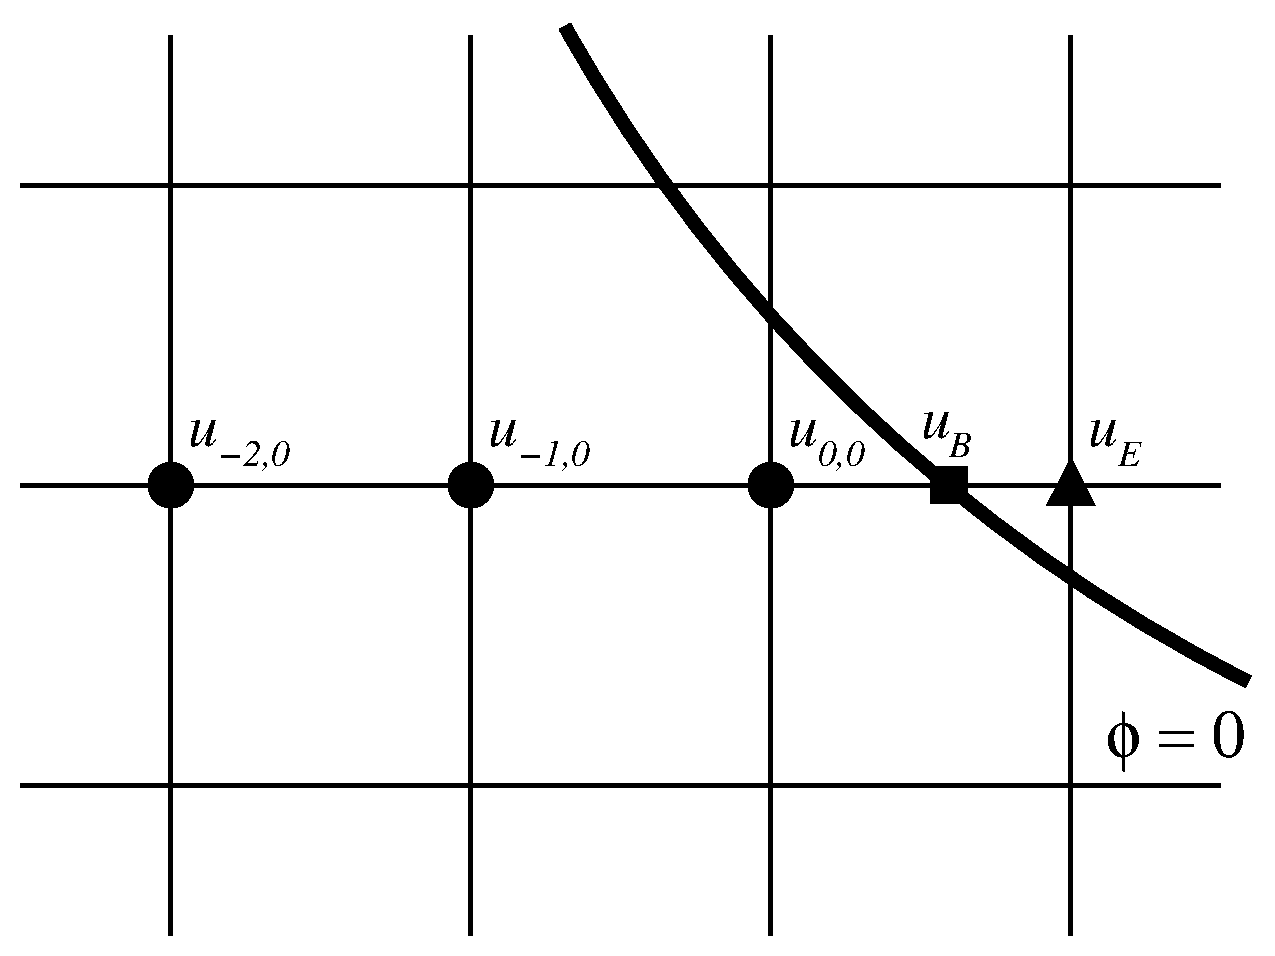
\includegraphics{figures/ghostcell_edge}} 
\ \ \ \ \ \ \ \ \ \ \ \ \ 
\scalebox{0.25}{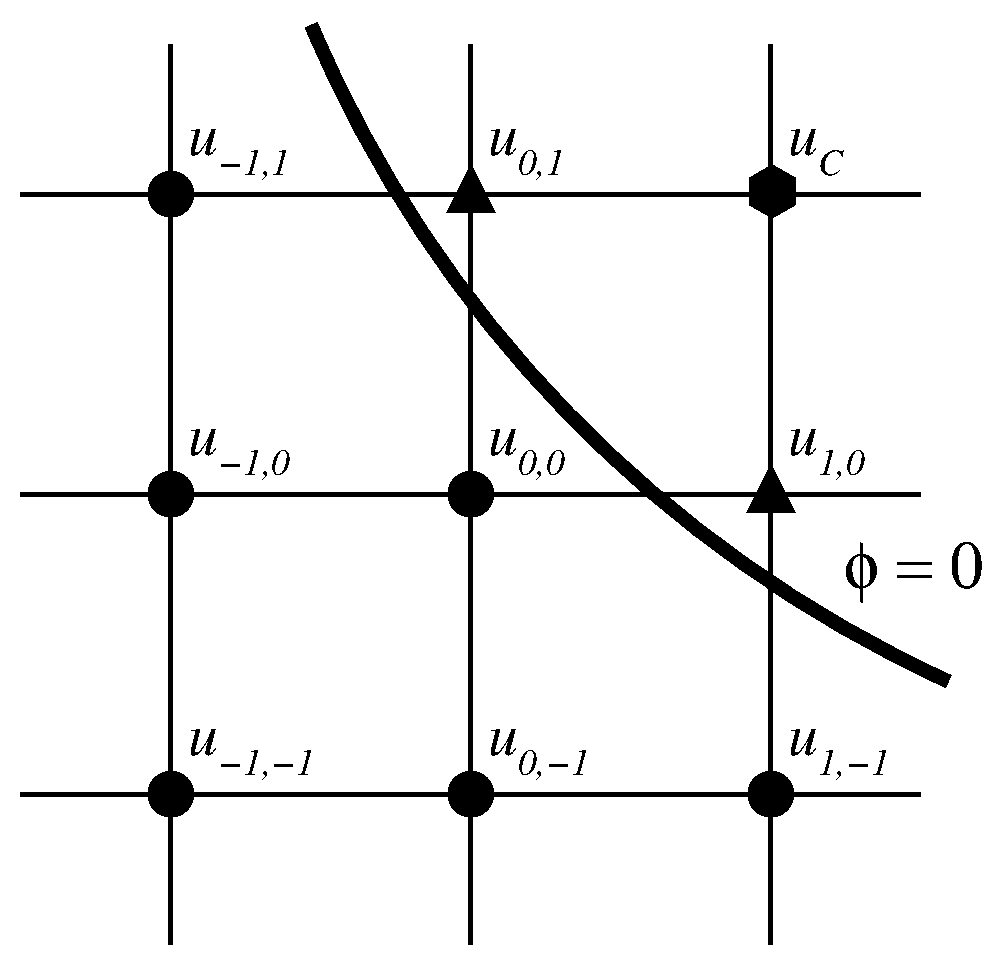
\includegraphics{figures/ghostcell_corner}}
\caption{Illustrations of edge (left) and corner (right) ghostcells.
The edge ghostcell, $u_E$, is filled by using cubic extrapolation of 
the value on the boundary, $u_B$, and values at three interior grid points.  
The corner ghostcells, $u_C$, is filled by using quadratic extrapolation 
of the values at interior grid points and neighboring edge ghost cells.
}
\label{fig:ghost_cells}
\end{center}
\end{figure}

The value in each edge ghost cell is set by using 1D, cubic extrapolation of 
the values of $u$ across the interface.  A cubic Lagrange extrapolant is 
constructed for each edge ghost cell using the point on the domain boundary 
where the zero level set of $\phi$ intersects the edge connecting the ghost 
cell to its nearest interior neighbor and three interior grid points along 
the line parallel to the same edge (see Figure~\ref{fig:ghost_cells}).  
The location of the point $u_B$ can be calculated by inverting the linear 
interpolant of $\phi$ that passes through the ghost cell and its nearest
interior neighbor.
Because the quality of the extrapolant deteriorates if the boundary point is 
too close to any of the interior grid 
points used to construct the Lagrange extrapolant, we follow 
\cite{gibou_2005} and choose the interior grid points so that the nearest
interior grid point is sufficiently far from the boundary point.  
Gibou~\etal suggest shifting the interpolation points by one grid point 
when the distance between the boundary point and the nearest interior grid 
point is less than $\dx^2$.  For the numerical scheme presented in this paper, 
thie threshold was too low.  We found that better results were obtained if 
we used a $O(\dx)$ threshold.

The values in corner ghost cells are set using 2D quadratic extrapolation
of the values of $u$ across the domain boundary \emph{and} the neighboring
edge ghost cells (see Figure~\ref{fig:ghost_cells}).  Notice that unlike
edge ghost cells, corner ghost cells only need to be 3rd-order accurate 
in order to obtain a 4th-order accurate solution.  The reason for this is ??.
*** KTC - FILL ME IN ***

To derive quadratic extrapolant at each corner ghost cell, we use a 
second-order Taylor series expansion around the nearest interior grid point,
$x_{0,0}$, and use finite differences to approximate all required partial 
derivatives.  For example, using central differences centered at $x_{0,0}$ for 
all partial derivatives, the quadratic extrapolant for the corner ghost cell 
shown in Figure~\ref{fig:ghost_cells} is
\bea
  u_C &=&  -u_{0,0} + \frac{1}{2} u_{-1,-1} 
      \nonumber \\
      &+& \frac{5}{4} u_{1,0} + \frac{5}{4} u_{0,1}
      - \frac{1}{4} u_{1,-1} - \frac{1}{4} u_{-1,1}
      - \frac{1}{4} u_{0,-1} - \frac{1}{4} u_{-1,0}
\eea
where $u_C$ and $u_{i,j}$ are as indicated in the figure.  Note that the 
stencil for the quadratic interpolant depends on the choice of finite 
difference approximation for the partial derivatives.  For the results 
presented in this paper, we use the above stencil (and its analogues for 
other positions of the ghost cell relative to the domain) to define the
quadratic extrapolant.  However, we obtained the same qualitative results 
when stencils based on other choices of finite difference approximations were
used.


\begin{figure}[htb]
\begin{center}
\scalebox{0.35}{\includegraphics{figures/diffusion_eqn_2d_starfish_domain_soln}} 
\scalebox{0.35}{\includegraphics{figures/diffusion_eqn_2d_starfish_domain_error}} 
\caption{Numerical solutions (left) and dominant error (right) for the 2D 
diffusion equation~(\ref{eq:??}) a starfish-shaped domain.  The numerical 
solution is computed at time $t = 0.1$ using forward Euler time stepping 
with an optimal time step and correction terms.  In the error plot, the dark 
regions represent points where the error in the solution is larger than 
$10$\% of the $L^\infty$ error of the solution.  Notice that the largest 
errors are concentrated near the boundaries of the mathematical domain.  To 
generate these results, the computational domain is taken to be 
$-1 < x,y < 1$ with 400 grid points in each direction.  The diffusion 
constant $D$ is set equal to $1/4$.  The source term is given by
$f(x,y,t) = 8 D \pi^2 \sin(2 \pi x) \sin(3 \pi y) 
            \exp\left(-5 D \pi^2 t\right)
          - 24 D \pi^2 \sin(5 \pi x) \sin(\pi y) 
            \exp \left(-2 D \pi^2 t \right).
$
The initial conditions are taken to be 
$u(x,y,0) = 1 + y/3 + x/2 + xy/4 
          + \sin(2 \pi x) \sin(3 \pi y) 
          - \sin(5 \pi x) \sin(\pi y)
$
and boundary conditions are imposed by using cubic and quadratic 
extrapolation of interior and boundary values to to fill edge and corner 
ghost cells, respectively.  Boundary values are obtained from the 
analytical solution
$u(x,y,t) = 1 + y/3 + x/2 + xy/4 
              + \sin(2 \pi x) \sin(3 \pi y) \exp(-5 D \pi^2 t) 
              - \sin(5 \pi x) \sin(\pi y) \exp(-2 D \pi^2 t)$.
The boundaries of the domains are represented by the zero-level 
set of the function
$\sqrt{x^2 + y^2} - \frac{3}{5} \left(1 + \frac{1}{2}\sin(5 \theta) \right)$, 
where $\theta = \mathtt{atan}\left( y/x \right)$.
}
\label{fig:diffusion_eqn_2d_starfish_domain}
\end{center}
\end{figure}

\begin{figure}[htb]
\begin{center}
\scalebox{0.35}{
  \includegraphics{figures/diffusion_eqn_2d_starfish_domain_error_vs_N}} 
\caption{Error analysis for four finite difference schemes 
for the 2D diffusion equation: forward Euler with optimal time step (circles), 
forward Euler with suboptimal time step (squares), 
(diamonds).  Using each method, we solve the 2D diffusion equation with 
$D = 1$ on the domain $0 < x < 1$ subject to the boundary conditions 
and the initial condition
$??$
The exact solution for this problem is
$u(x,t) = ??$
The $L^\infty$ error is plotted against the grid spacing $\dx$ for each 
method.  Note that the errors for the forward Euler with suboptimal time 
step and Crank-Nicholson schemes lie almost directly on top of each other
at the resolution of the figures.
}
\label{fig:diffusion_eqn_2d_starfish_error}
\end{center}
\end{figure}


\subsubsection{Generalization to Higher Dimensional Problems}
** COMPLEXITY OF EXTRAPOLATION DEPENDS ON CHOICE OF DISCRETIZATION FOR LAPLACIAN **

** PATRA AND KARTTUNEN GIVE ISOTROPIC STENCILS FOR 3D **


\subsubsection{Weakly Anisotropic Diffusivity Tensor}
can use unequal grid spacing when the diffusivity tensor is diagonlizable 
(i.e. normal) and the eigenvalues are unequal.  first transform to coordinate
system of principle axes then rescale problem.



\section{\label{sec:summary} Summary} 
While somewhat tedious, analyzing higher-order errors can suggest simple 
modifications to numerical methods that greatly improve their accuracy.  
Symbolic mathematics tools can be helpful to make this easier.

Optimal time step selection is not applicable to all PDEs.  ...


% ACKNOWLEDGMENTS
\section*{Acknowledgments}
The author gratefully acknowledges the support of the Institute for 
High-Performance Computing (IHPC) in Singapore and Vitamin D, Inc.
The author would like to thanks P. Fok and ?? for enlightening discussions 
and suggestions on the manuscript.

\bibliography{optimal_time_steps_for_pdes}

\end{document}
